% IDM-Viz research paper -- main file (IEEEtran journal template)
\documentclass[journal]{IEEEtran}

\usepackage[T1]{fontenc}
\usepackage{amsmath,amssymb,amsfonts}
\usepackage{graphicx}
\usepackage{booktabs}
\usepackage{multirow}
\usepackage{array}
\usepackage{tabularx}
\usepackage[table]{xcolor}
\usepackage{tikz}
\usetikzlibrary{positioning,arrows.meta,fit,backgrounds,shapes.geometric,shapes.misc,calc,shadows}
\usepackage{pgfplots}
\pgfplotsset{compat=1.18}
\usepgfplotslibrary{groupplots,fillbetween,colormaps}
\usepackage{algorithm}
\usepackage{algpseudocode}
\usepackage{cite}
\usepackage{url}
\usepackage[hidelinks]{hyperref}

% ---------------------------------------------------------------- notation
\newcolumntype{L}[1]{>{\raggedright\arraybackslash}p{#1}}
\newcommand{\Aref}{A_{\mathrm{ref}}}
\newcommand{\Ahat}{\hat{A}}
\newcommand{\concern}{\kappa}
\newcommand{\idm}{IDM-Viz}

% ---------------------------------------------------------------- house style for all figures
% Okabe--Ito colour-blind-safe palette
\definecolor{c1}{HTML}{0072B2}   % blue
\definecolor{c2}{HTML}{D55E00}   % vermillion
\definecolor{c3}{HTML}{009E73}   % bluish green
\definecolor{c4}{HTML}{CC79A7}   % reddish purple
\definecolor{c5}{HTML}{E69F00}   % orange
\definecolor{c6}{HTML}{56B4E9}   % sky blue
\definecolor{cgray}{HTML}{6E6E6E}
\definecolor{cink}{HTML}{1F2933}
\pgfplotsset{
  idm/.style={
    axis lines=left, axis line style={cink!70, line width=0.5pt},
    tick style={cink!70, line width=0.4pt}, tick align=outside, major tick length=2pt,
    every tick label/.append style={font=\scriptsize, text=cink},
    label style={font=\footnotesize, text=cink},
    title style={font=\footnotesize\bfseries, text=cink, yshift=-2pt},
    ymajorgrids, grid style={cink!9, line width=0.35pt},
    legend style={font=\scriptsize, draw=cink!20, fill=white, fill opacity=0.92, text opacity=1, rounded corners=1pt, inner sep=1.5pt},
    legend cell align=left,
    every axis plot/.append style={line join=round},
  },
}

\begin{document}

% ---------------------------------------------------------------
\title{IDM-Viz: Label-Safe, Impact-Aware\\Drift Monitoring for Tabular Data Streams\\with Delayed Labels}

% IEEE-style author block: one column per author (name, affiliation, e-mail)
\author{%
\begin{tabular}{c@{\hspace{2.5em}}c}
\large Ahmed Bilal Azhar & \large Umar Behram \\[2pt]
\normalsize\itshape Department of AI and Data Science & \normalsize\itshape Department of AI and Data Science \\
\normalsize\itshape FAST-NUCES, Islamabad, Pakistan & \normalsize\itshape FAST-NUCES, Islamabad, Pakistan \\
\normalsize i232581@isb.nu.edu.pk & \normalsize i232604@isb.nu.edu.pk
\end{tabular}%
\thanks{A.~B.~Azhar (23I-2581) and U.~Behram (23I-2604) are BS Data Science students at the
National University of Computer and Emerging Sciences (FAST-NUCES), Islamabad. This work
was prepared for the Data Analysis and Visualization course. Code, locked protocols and
results: \url{https://github.com/ahmedbilalazhar/ml-data-drift-visualization} (commit \texttt{78abb9f}).}}

\markboth{Bilal and Umar: Label-Safe, Impact-Aware Drift Monitoring}%
{Bilal and Umar: Label-Safe, Impact-Aware Drift Monitoring}

\maketitle

% ---------------------------------------------------------------
\begin{abstract}
Deployed classifiers are usually monitored through input drift tests, while the labels
that reveal actual harm arrive late. Existing detectors and drift visualizations rarely
test whether an alarm reflects lost accuracy, or when labels arrive. This paper presents \idm{}, a framework that keeps a
label-free input channel (Holm-corrected Kolmogorov--Smirnov tests, a correlation-change
statistic and feature ranking) separate from an impact channel (isotonic-calibrated
average confidence with a Poisson-binomial interval and a harm-concern score). A broker
releases ground truth only after a set delay. The framework was evaluated on 360 controlled synthetic
streams (4.32 million rows), a 1,500-seed replication and three natural streams (UCI
gas sensor, ELEC2, NOAA weather). Marginal shifts were detected in 30/30 seeds. When
only $P(Y\mid X)$ changed, none of 1,205 harmful batches received a concern flag, and
1,140 of them received no input alarm either. After onset, mean estimated accuracy was
0.723 against a realised 0.370. The correlation statistic detected a dependence-only
change in 30/30 seeds versus 16/30 for the KS tests (+46.7 points). Combined with KS,
however, it raised stationary alarms from 0.83 to 2.37 per 24 batches. Recalibration on
released labels cut gas-sensor estimation error by 68.9\% (MAE 0.545 to 0.169), but did
not help on ELEC2 (0.059 to 0.063). Monitor features lowered the Brier score of a harm
forecaster by 27.9\% over a time-only model on known laws. On a held-out law, time alone
kept the highest AUC. Input drift alarms are therefore not reliable harm signals, and
until labels are released some harm cannot be detected from unlabelled evidence.
\end{abstract}

% ---------------------------------------------------------------
\begin{IEEEkeywords}
Concept drift, data drift monitoring, delayed labels, label-free performance estimation, confidence calibration, visual analytics.
\end{IEEEkeywords}

% ---------------------------------------------------------------
\section{Introduction}
\label{sec:intro}

\IEEEPARstart{M}{achine-learning} models are trained on historical data and then used
on data that keep changing. When the joint distribution $P(X,Y)$ moves away from the
training distribution, accuracy can fall without any visible error~\cite{gama2014survey,lu2019learning,webb2016characterizing}.
Practitioners usually respond by monitoring the model's \emph{inputs}: a
two-sample test compares a recent window with a reference window, and an alarm is
raised when the difference is significant~\cite{rabanser2019failing,gretton2012kernel,lukats2025benchmark}.
Monitoring inputs is attractive because labels are expensive and often arrive days or
weeks after the prediction is made~\cite{grzenda2020delayed,zliobaite2010change}.

Input monitoring answers a narrower question than the one operators need. A shift in
an irrelevant feature or a seasonal fluctuation can trigger an alarm while accuracy is
unchanged. A change confined to the labelling rule $P(Y\mid X)$ can destroy accuracy
without any change in the inputs. In that case accuracy is not identifiable from
unlabelled data alone~\cite{bayram2022concept,lipton2018detecting}. Confidence-based
estimators of accuracy~\cite{garg2022atc,guillory2021predicting,kivimaki2025confidence}
and drift explainers~\cite{hinder2024surveyB,szucs2025dde} add useful evidence, but
each is usually evaluated in isolation. Visual-analytics systems for drift~\cite{yang2020driftvis,wang2020conceptexplorer}
display that evidence but are rarely scored against verified harm. Their displays also
seldom show which outcomes were still unknown when a decision was made.

\textbf{Research gap.} No study known to the authors evaluates, \emph{in one
label-safe pipeline}, how input alarms, feature-level evidence and calibrated accuracy
estimates relate to verified model harm while labels arrive with an explicit delay.
None also reports where this combination fails. The gap is empirical as well as
architectural. Most evaluations let the monitor (or the evaluator) see labels
earlier than a deployed system could, and they report detection rates without
reporting the harm that went unflagged.

This paper closes that gap with \idm{} (Impact-aware Drift Monitoring with Visual
explanation) and an evaluation protocol whose settings were locked before each run. The contributions are:
\begin{itemize}
  \item A label-safe architecture that separates label-free input evidence from
  calibrated impact evidence and releases ground truth only through a delay-enforcing
  broker (Section~\ref{sec:method}).
  \item A controlled benchmark with known change type and known harm, covering two
  learners, three delays and a 1,500-seed replication (Sections~\ref{sec:setup}--\ref{sec:results}).
  \item Quantified failure modes: under conditional-only change none of 1,205 harmful
  batches is flagged, and closing the dependence blind spot nearly triples false
  alarms (Sections~\ref{sec:results} and~\ref{sec:ablation}).
  \item Evidence from three natural streams and a prospective harm forecaster on where
  delayed labels help and where they do not (Section~\ref{sec:results}).
  \item An aligned evidence view and a fully traceable, rerun-verified artefact
  (Sections~\ref{sec:method} and~\ref{sec:decl}).
\end{itemize}

The remainder of the paper is organised as follows.
Section~\ref{sec:related} reviews related work by theme. Section~\ref{sec:method}
formulates the problem and describes \idm{}. Section~\ref{sec:setup} gives the
experimental setup, and Section~\ref{sec:results} the results. Section~\ref{sec:comparison}
compares the work with its base papers, and Section~\ref{sec:ablation} reports
ablations. Section~\ref{sec:discussion} discusses implications and limitations, and
Section~\ref{sec:conclusion} concludes.\begin{itemize}
  \item A label-safe architecture that separates label-free input evidence from
  calibrated impact evidence and releases ground truth only through a delay-enforcing
  broker (Section~\ref{sec:method}).
  \item A controlled benchmark with known change type and known harm, covering two
  learners, three delays and a 1,500-seed replication (Sections~\ref{sec:setup}--\ref{sec:results}).
  \item Quantified failure modes: under conditional-only change, none of 1,205 harmful
  batches is flagged, and closing the dependence blind spot nearly triples false
  alarms (Sections~\ref{sec:results},~\ref{sec:ablation}).
  \item Evidence from three natural streams and a prospective harm forecaster, which
  shows where delayed labels help and where they do not (Section~\ref{sec:results}).
  \item An aligned evidence view and a fully traceable, rerun-verified artefact
  (Sections~\ref{sec:method},~\ref{sec:decl}).
\end{itemize}

The remainder of the paper is organised as follows.
Section~\ref{sec:related} reviews related work by theme. Section~\ref{sec:method}
formulates the problem and describes \idm{}. Section~\ref{sec:setup} gives the
experimental setup, and Section~\ref{sec:results} the results. Section~\ref{sec:comparison}
compares the work with its base papers, and Section~\ref{sec:ablation} reports
ablations. Section~\ref{sec:discussion} discusses implications and limitations, and
Section~\ref{sec:conclusion} concludes.

% ---------------------------------------------------------------
\section{Related Work}
\label{sec:related}

\subsection{Unsupervised Drift Detection}
Two-sample tests are the standard label-free monitor. Univariate KS tests with a
multiple-testing correction remain strong baselines for tabular shift
detection~\cite{rabanser2019failing}. Kernel tests such as MMD target multivariate
differences~\cite{gretton2012kernel}. ADWIN maintains an adaptive window over a
stream of real values, such as errors, and detects changes in their mean~\cite{bifet2007adwin}.
ADWIN-U extends adaptive windowing to the unsupervised setting~\cite{assis2025adwinu}.
DriftLens models deep embeddings per label with Gaussians and measures their Fréchet
distance from a reference window, which gives real-time detection and drift curves on
unstructured data~\cite{greco2025driftlens,greco2024driftlensdemo}. Recent benchmarks
show that unsupervised detectors behave very differently on real streams, where onset
truth is rarely available~\cite{lukats2025benchmark,souza2020challenges,cerqueira2026framework}.
Gower-Winter et al.\ argue that window-based detection is ill-posed without
assumptions~\cite{gowerwinter2026window}. Uncertainty-based, label-free and conformal detectors continue to be
proposed~\cite{lu2025pudd,tan2025flexible,eliades2025conformal}.
\emph{Strength:} they need no labels, scale to many features and come with
calibrated false-alarm control. \emph{Limitation for this setting:} they report
alarms, and whether an alarm coincides with lost accuracy lies outside their
evaluation target.

\subsection{Drift Localization and Explanation}
Hinder et al.\ survey how drift can be located and explained and give model-based
explanations of drift~\cite{hinder2024surveyA,hinder2024surveyB,hinder2023modelbased}.
Regional drift detection localizes change in feature space~\cite{liu2017regional}.
The domino drift effect (DDE) infers drift in unmonitored features from correlated,
already-drifting monitored features, which saves per-feature detectors in high
dimension~\cite{szucs2025dde}. Causal explanations of drift aim at actionable
attribution~\cite{komnick2026causal}. In medical imaging, shift identification is used
to support root-cause analysis~\cite{roschewitz2026shiftid}.
\emph{Strength:} they turn an alarm into an inspectable hypothesis and, in the case of
DDE, cut monitoring cost in high dimension. \emph{Limitation:} explanations describe
distributional change. They are seldom tested on whether the explained change caused
the loss of performance, and they cannot address changes that leave $P(X)$ untouched.

\subsection{Performance Estimation without Labels}
Average confidence, the ATC threshold estimator and difference-of-confidence estimate
accuracy under shift from unlabelled data~\cite{garg2022atc,guillory2021predicting}.
Agreement-on-the-line estimates accuracy from the agreement between
models~\cite{baek2022agreement}. Kivimäki et al.\ study confidence-based estimators for
model monitoring~\cite{kivimaki2025confidence}. Label-shift correction assumes a fixed
$P(X\mid Y)$~\cite{lipton2018detecting}. All of these depend on calibration, which
often degrades under shift~\cite{guo2017calibration,zadrozny2002transforming,platt2000probabilities}.
Performance-aware detectors~\cite{bayram2022concept} and risk monitors cover the case
where labels arrive eventually~\cite{timans2025risk,zhang2026pprm,pouget2025suitability}.
\emph{Strength:} they target accuracy, the quantity operators care about, rather than
a distance between distributions. \emph{Limitation:} they are usually scored offline
on a fixed target set, and the time at which labels are released is rarely modelled.

\subsection{Delayed Labels and Adaptation}
Evaluating stream learners under delayed labels changes their measured
performance~\cite{grzenda2020delayed}, and some changes are undetectable until labels
arrive~\cite{zliobaite2010change}. PRODEM targets degradation detection with delayed
labels in fraud prediction~\cite{sethi2026prodem}. Proactive Hoeffding trees anticipate
incremental drift so that the model adapts before it degrades~\cite{guerrerocano2026proactive}.
Adaptation surveys organise reactive and proactive strategies~\cite{gama2014survey,lu2019learning}.
\emph{Strength:} they measure accuracy directly over time. \emph{Limitation:}
adaptation studies typically assume immediate (prequential) labels, and they rarely
compare update policies at matched label and refit budgets.

\subsection{Visual Analytics for Drift}
DriftVis~\cite{yang2020driftvis} and ConceptExplorer~\cite{wang2020conceptexplorer}
support interactive diagnosis of concept drift. Coordinated multiple views are an
established design for linking evidence across panels~\cite{roberts2007cmv}, and visual
analytics for deep learning has been surveyed~\cite{hohman2019visual}. Drift
visualization for specific learners has also been proposed~\cite{galmeanu2024svmviz}.
\emph{Strength:} they make drift legible to analysts. \emph{Limitation:} they are
evaluated mainly through case studies, and their displays rarely encode which outcomes
were still unknown at the time of a decision.

\subsection{Positioning}
Table~\ref{tab:related} summarises representative studies along the dimensions that
matter here. \idm{} does not propose a new detector. Its novelty lies in the
\emph{combination}: label-free input evidence and calibrated impact evidence are scored
against verified harm, under an enforced release delay, on streams where the
conditional law changes without any input change.

\begin{table*}[t]
\centering
\caption{Representative related studies organised by theme. \checkmark: addressed; --: not addressed in the evaluated setting.}
\label{tab:related}
\setlength{\tabcolsep}{3pt}
\footnotesize
\begin{tabular}{L{3.4cm}L{2.3cm}ccccL{4.3cm}}
\toprule
Study & Theme & Label-free & Delay modelled & Harm-linked & Explanation / view & Limitation for delayed-label harm monitoring \\
\midrule
Rabanser et al.~\cite{rabanser2019failing} & shift detection & \checkmark & -- & -- & -- & alarms not scored against accuracy loss \\
Greco et al.\ (DriftLens)~\cite{greco2025driftlens} & embedding drift & \checkmark & -- & -- & \checkmark & deep unstructured data; label-conditioned baselines \\
Lukats et al.~\cite{lukats2025benchmark} & detector benchmark & \checkmark & -- & -- & -- & real streams lack onset and harm truth \\
Sz\H{u}cs \& N\'emeth (DDE)~\cite{szucs2025dde} & drift localization & \checkmark & -- & -- & \checkmark & needs co-drifting correlated features \\
Hinder et al.~\cite{hinder2024surveyB} & drift explanation & \checkmark & -- & -- & \checkmark & descriptive, not causal \\
Garg et al.\ (ATC)~\cite{garg2022atc} & accuracy estimation & \checkmark & -- & \checkmark & -- & offline target sets; calibration-dependent \\
Kivim\"aki et al.~\cite{kivimaki2025confidence} & accuracy estimation & \checkmark & -- & \checkmark & -- & assumes calibration transfers under shift \\
Grzenda et al.~\cite{grzenda2020delayed} & delayed evaluation & -- & \checkmark & \checkmark & -- & evaluation protocol, not a monitor \\
Guerrero Cano et al.~\cite{guerrerocano2026proactive} & proactive adaptation & -- & -- & \checkmark & -- & prequential labels; incremental drift \\
Yang et al.\ (DriftVis)~\cite{yang2020driftvis} & visual analytics & \checkmark & -- & -- & \checkmark & case-study evaluation \\
\midrule
\textbf{\idm{} (this work)} & monitoring + evaluation & \checkmark & \checkmark & \checkmark & \checkmark & synthetic-heavy; no analyst study \\
\bottomrule
\end{tabular}
\end{table*}

% ---------------------------------------------------------------
\section{Proposed Methodology}
\label{sec:method}

\subsection{Problem Formulation}
\label{sec:formulation}
A binary classifier $f:\mathbb{R}^{M}\rightarrow[0,1]$ on $M$ input features is
trained once and then frozen. It returns $p(x)=\Pr_f(Y{=}1\mid x)$, the prediction
$\hat{y}=\mathbb{I}\{p(x)\ge 0.5\}$ and the raw confidence
$s(x)=\max\{p(x),1-p(x)\}$. Before deployment, three disjoint labelled historical
partitions are drawn: a training set $\mathcal{D}_{\mathrm{tr}}$, a
correctness-calibration set $\mathcal{D}_{\mathrm{cal}}$ and a reference set
$\mathcal{D}_{\mathrm{ref}}$. The historical reference accuracy
$\Aref$ is the accuracy of $f$ on $\mathcal{D}_{\mathrm{ref}}$.
After deployment, unlabelled inputs arrive in batches
$B_t=\{x_{t,1},\dots,x_{t,n}\}$, $t=1,\dots,T$, of size $n$. The realised batch
accuracy $A_t=\frac{1}{n}\sum_{i}\mathbb{I}\{\hat{y}_{t,i}=y_{t,i}\}$ cannot be
computed when $B_t$ arrives, because its labels are released only after a delay of
$d\in\mathbb{N}$ batches. A batch is \emph{harmful} when
\begin{equation}
H_t=\mathbb{I}\{A_t<\Aref-\delta\},\qquad \delta=0.05.
\label{eq:harm}
\end{equation}
At every clock $t$ the monitor must report, from $B_t$ and the labels released so
far, (i) whether the input distribution has changed, (ii) which features carry the
change, (iii) an estimate $\Ahat_t$ of $A_t$ with an uncertainty statement, and
(iv) whether $H_t=1$ is likely. Because $P(X)$ can stay fixed while $P(Y\mid X)$
changes, (i) and (iv) are separate targets. The framework is required to keep them
separate and to show when (iv) cannot be supported by unlabelled evidence.

\subsection{Architecture Overview}
Fig.~\ref{fig:arch} shows the \idm{} pipeline. All artefacts are fitted on
historical data and then frozen. Two evidence channels run in parallel on each
batch: a label-free \emph{input channel} (detection and localization) and an
\emph{impact channel} (calibrated accuracy estimation and a harm-concern score).
A label-release broker is the only component that holds ground truth. It
reveals labels to a verification ledger strictly according to the delay schedule.
An aligned evidence view shows both channels and the verified outcomes on one
shared batch axis. It leaves a cell empty while its label is unreleased and never
imputes the value. The numbered badges 1--6 in Fig.~\ref{fig:arch} mark the stages
described below, and Table~\ref{tab:notation} in the appendix lists all symbols.

\begin{figure*}[t]
\centering
\resizebox{\textwidth}{!}{% Architecture diagram of IDM-Viz (TikZ; contains no data values).
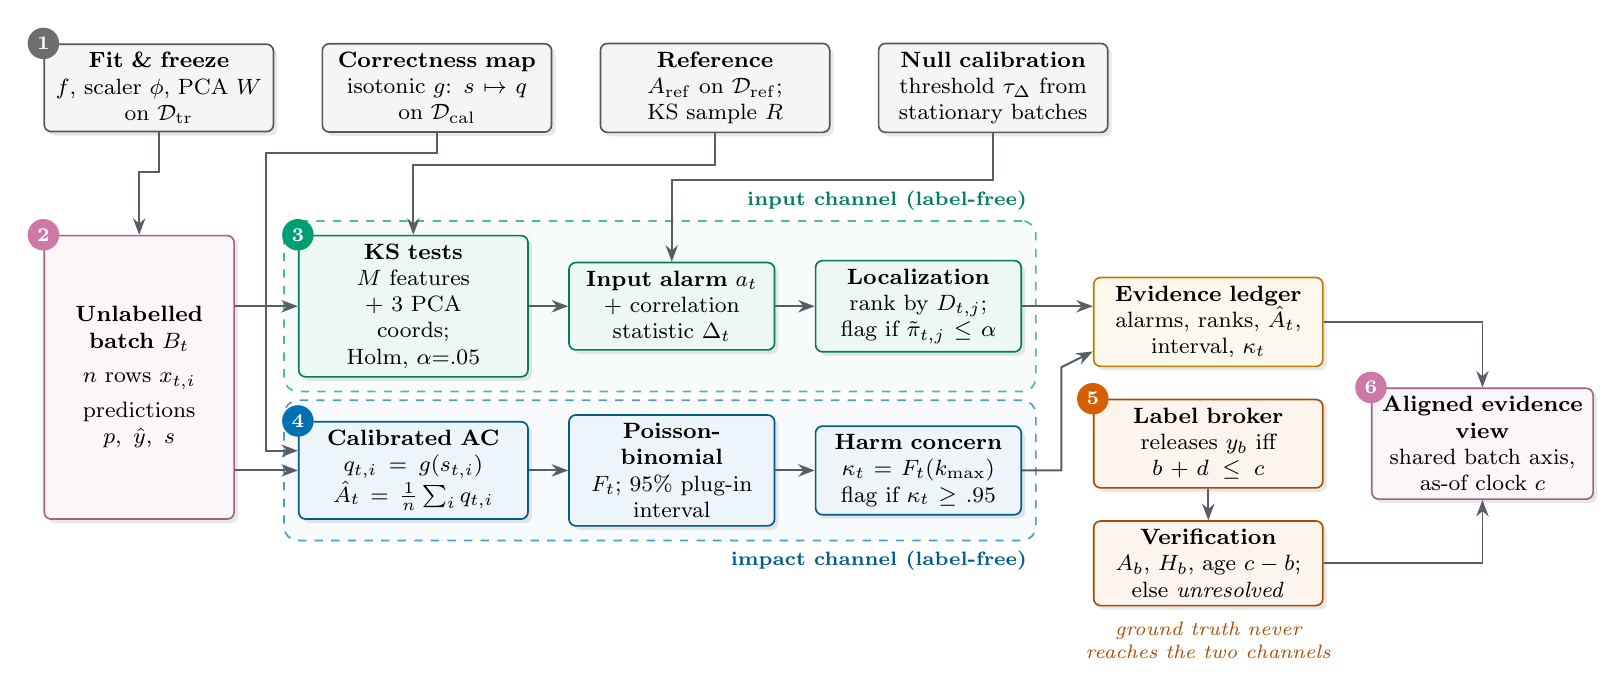
\begin{tikzpicture}[
  font=\footnotesize,
  >={Stealth[length=2.1mm]},
  box/.style={draw=#1!80!black, line width=0.6pt, rounded corners=2.5pt, align=center, fill=#1!7, minimum height=10mm, inner sep=3pt, drop shadow={opacity=0.18, shadow xshift=0.5mm, shadow yshift=-0.5mm}},
  box/.default=c1,
  lane/.style={draw=#1!70, dashed, line width=0.6pt, rounded corners=5pt, inner sep=5pt, fill=#1!3},
  arr/.style={->, line width=0.7pt, draw=cink!75},
  lab/.style={font=\scriptsize\bfseries, text=#1!80!black},
  badge/.style={circle, fill=#1, text=white, font=\scriptsize\bfseries, inner sep=0.8pt, minimum size=4mm},
]
% --- frozen artefacts (top row)
\node[box=cgray, text width=27mm] (fit) {\textbf{Fit \& freeze}\\$f$, scaler $\phi$, PCA $W$\\on $\mathcal{D}_{\mathrm{tr}}$};
\node[box=cgray, text width=27mm, right=6mm of fit] (cal) {\textbf{Correctness map}\\isotonic $g$: $s\mapsto q$\\on $\mathcal{D}_{\mathrm{cal}}$};
\node[box=cgray, text width=27mm, right=6mm of cal] (ref) {\textbf{Reference}\\$\Aref$ on $\mathcal{D}_{\mathrm{ref}}$;\\KS sample $R$};
\node[box=cgray, text width=27mm, right=6mm of ref] (null) {\textbf{Null calibration}\\threshold $\tau_\Delta$ from\\stationary batches};

% --- stream
\node[box=c4, text width=22mm, below=13mm of fit.south west, anchor=north west, minimum height=36mm] (batch) {\textbf{Unlabelled}\\\textbf{batch $B_t$}\\[3pt] $n$ rows $x_{t,i}$\\[3pt] predictions\\$p,\ \hat{y},\ s$};

% --- input channel
\node[box=c3, text width=27mm, right=8mm of batch.north east, anchor=north west] (ks) {\textbf{KS tests}\\$M$ features + 3 PCA\\coords; Holm, $\alpha{=}.05$};
\node[box=c3, text width=24mm, right=5mm of ks] (alarm) {\textbf{Input alarm} $a_t$\\+ correlation\\statistic $\Delta_t$};
\node[box=c3, text width=24mm, right=5mm of alarm] (loc) {\textbf{Localization}\\rank by $D_{t,j}$;\\flag if $\tilde\pi_{t,j}\le\alpha$};

% --- impact channel
\node[box=c1, text width=27mm, right=8mm of batch.south east, anchor=south west] (q) {\textbf{Calibrated AC}\\$q_{t,i}=g(s_{t,i})$\\$\Ahat_t=\frac{1}{n}\sum_i q_{t,i}$};
\node[box=c1, text width=24mm, right=5mm of q] (pb) {\textbf{Poisson-binomial}\\$F_t$; 95\% plug-in\\interval};
\node[box=c1, text width=24mm, right=5mm of pb] (kap) {\textbf{Harm concern}\\$\concern_t=F_t(k_{\max})$\\flag if $\concern_t\ge .95$};

% --- lanes
\begin{scope}[on background layer]
\node[lane=c3, fit=(ks)(alarm)(loc)] (laneA) {};
\node[lane=c1, fit=(q)(pb)(kap)] (laneB) {};
\end{scope}
\node[lab=c3, anchor=south east] at (laneA.north east) {input channel (label-free)};
\node[lab=c1, anchor=north east] at (laneB.south east) {impact channel (label-free)};

% --- ledger, broker, verification, view
\node[box=c5, text width=27mm, right=9mm of loc.east, anchor=west, yshift=-2mm] (ledger) {\textbf{Evidence ledger}\\alarms, ranks, $\Ahat_t$,\\interval, $\concern_t$};
\node[box=c2, text width=27mm, below=4mm of ledger] (broker) {\textbf{Label broker}\\releases $y_b$ iff\\$b+d\le c$};
\node[box=c2, text width=27mm, below=4mm of broker] (verif) {\textbf{Verification}\\$A_b$, $H_b$, age $c-b$;\\else \emph{unresolved}};
\node[box=c4, text width=26mm, right=6mm of broker] (view) {\textbf{Aligned evidence}\\\textbf{view}\\shared batch axis,\\as-of clock $c$};

% --- arrows
\draw[arr] (fit.south) -- ++(0,-5mm) -| (batch.north);
\draw[arr] (batch.east |- ks.west) -- (ks.west);
\draw[arr] (ks) -- (alarm);
\draw[arr] (alarm) -- (loc);
\draw[arr] (batch.east |- q.west) -- (q.west);
\draw[arr] (q) -- (pb);
\draw[arr] (pb) -- (kap);
\draw[arr] (ref.south) -- ++(0,-4mm) -| (ks.north);
\draw[arr] (null.south) -- ++(0,-6mm) -| (alarm.north);
\draw[arr] (cal.south) -- ++(0,-2.5mm) -| ($(batch.east)+(4mm,0)$) |- ([yshift=2.5mm]q.west);
\draw[arr] (loc.east) -- (loc.east -| ledger.west);
\draw[arr] (kap.east) -| ([xshift=-4mm]ledger.south west) -- ([yshift=2mm]ledger.south west);
\draw[arr] (broker) -- (verif);
\draw[arr] (ledger.east) -| (view.north);
\draw[arr] (verif.east) -| (view.south);
\node[font=\scriptsize\itshape, text=c2!80!black, below=0.8mm of verif, text width=32mm, align=center] {ground truth never reaches the two channels};

% --- stage badges
\node[badge=cgray] at (fit.north west) {1};
\node[badge=c4] at (batch.north west) {2};
\node[badge=c3] at (ks.north west) {3};
\node[badge=c1] at (q.north west) {4};
\node[badge=c2] at (broker.north west) {5};
\node[badge=c4] at (view.north west) {6};
\end{tikzpicture}
}
\caption{\idm{} architecture. The classifier, scaler, PCA basis, isotonic
correctness map and reference sample are fitted on historical partitions and then
frozen (top). Each unlabelled batch feeds two independent channels. The input
channel applies per-feature and per-PCA-coordinate Kolmogorov--Smirnov tests with Holm
correction, an optional pairwise-correlation statistic and a feature ranking. The
impact channel computes calibrated average confidence, a plug-in Poisson-binomial
interval and a harm-concern score. Ground-truth labels are held by a release broker
and the labels of source batch $b$ reach the verification ledger only when
$b+d\le c$, where $c$ is the current clock. The aligned evidence view
reads the ledger as of a chosen clock $c$.}
\label{fig:arch}
\end{figure*}

\subsection{Input Channel: Detection}
\label{sec:detection}
Let $z=\phi(x)$ denote the standardized input. Let
$u=W^{\top}z\in\mathbb{R}^{3}$ be its projection on the first three principal
components, which are fitted on $\mathcal{D}_{\mathrm{tr}}$. For every original
feature and each of the three coordinates $u_1,u_2,u_3$, indexed jointly by
$j\in\{1,\dots,m\}$ with $m=M+3$, a two-sample
Kolmogorov--Smirnov (KS) statistic~\cite{massey1951ks} compares $B_t$ with a frozen
reference sample $R$ of $1{,}000$ historical rows:
\begin{equation}
D_{t,j}=\sup_{v}\bigl|\hat{F}_{B_t,j}(v)-\hat{F}_{R,j}(v)\bigr|.
\end{equation}
The $m$ resulting $p$-values $\pi_{t,j}$ are adjusted with Holm's step-down
procedure~\cite{holm1979}: with the $p$-values sorted in ascending order,
$\tilde{\pi}_{t,(i)}=\min\{1,\max_{l\le i}(m-l+1)\pi_{t,(l)}\}$.
The input alarm is $a_t=\mathbb{I}\{\min_j\tilde{\pi}_{t,j}\le\alpha\}$ with
$\alpha=0.05$. The PCA coordinates take the place of the autoencoder latent space
proposed in Phase~2 (Section~\ref{sec:changes}). They add a small amount of joint
evidence, but they do not reproduce a learned embedding detector such as
DriftLens~\cite{greco2025driftlens}.

Marginal tests cannot see a change that alters only feature dependence. An
optional \emph{dependence statistic} therefore tracks the largest absolute change in
pairwise Pearson correlation:
\begin{equation}
\Delta_t=\max_{i<j}\bigl|\hat{\rho}_{B_t}(i,j)-\hat{\rho}_{R}(i,j)\bigr|,
\label{eq:dep}
\end{equation}
where $\hat{\rho}_{B}(i,j)$ is the sample Pearson correlation of features $i$ and $j$
in sample $B$, and alarms when $\Delta_t>\tau_\Delta$. The threshold $\tau_\Delta$ is the empirical
$95$th percentile of $\Delta$ over stationary development batches. The arg-max pair
is reported as dependence evidence. It is descriptive, not causal.

\subsection{Input Channel: Localization}
Features are ranked by $D_{t,j}$ in descending order. A feature is \emph{flagged}
only when $\tilde{\pi}_{t,j}\le\alpha$. When the set $S$ of changed features is known,
which is the case in synthetic marginal shifts, localization is scored by
$\mathrm{P@1}=\mathbb{I}\{r_1\in S\}$ and
$\mathrm{R@3}=|\{r_1,r_2,r_3\}\cap S|/|S|$, where $r_k$ is the $k$-th ranked
feature. Both scores are undefined when $S=\emptyset$, as under conditional-only or
dependence-only change. The ranking is a description of distributional change and
does not identify a cause.

\subsection{Impact Channel: Calibrated Accuracy Estimation}
\label{sec:impact}
The impact channel follows the confidence-based performance estimators studied by
Kivim\"aki et al.~\cite{kivimaki2025confidence} and the average-confidence and ATC
literature~\cite{garg2022atc,guillory2021predicting}. It does not claim a new
estimator. Its contribution is to run the estimator behind a release broker and to
score it against verified harm. The raw confidence $s$ of a classifier is often
miscalibrated~\cite{guo2017calibration}, so \idm{} fits a monotone correctness map
$g:[0.5,1]\rightarrow[0,1]$ on $\mathcal{D}_{\mathrm{cal}}$ by isotonic
regression~\cite{zadrozny2002transforming}:
\begin{equation}
g=\arg\min_{\psi\ \text{non-decreasing}}\ \sum_{i\in\mathcal{D}_{\mathrm{cal}}}
\bigl(\mathbb{I}\{\hat{y}_i=y_i\}-\psi(s_i)\bigr)^{2}.
\label{eq:iso}
\end{equation}
Equation~\eqref{eq:iso} is the only learning objective in the monitor. The frozen
classifier is not retrained. Each prediction receives a calibrated correctness
probability $q_{t,i}=g(s_{t,i})$. The batch accuracy estimate is the calibrated
average confidence (AC)
\begin{equation}
\Ahat_t=\frac{1}{n}\sum_{i=1}^{n}q_{t,i}.
\label{eq:ac}
\end{equation}
An estimator is scored by $|\Ahat_t-A_t|$ once $A_t$ has been verified.

\subsection{Impact Channel: Interval and Harm Concern}
Treating the $q_{t,i}$ as known, independent Bernoulli success probabilities gives
a plug-in Poisson-binomial model for the number of correct predictions,
$K_t=\sum_iZ_{t,i}$ with $Z_{t,i}\sim\mathrm{Bernoulli}(q_{t,i})$. Its probability
mass function is computed exactly by the recursion
$P_i(k)=(1-q_{t,i})P_{i-1}(k)+q_{t,i}P_{i-1}(k-1)$~\cite{hong2013poibin}.
With $F_t$ the resulting distribution function, the $95\%$ plug-in interval for
$A_t$ is $[F_t^{-1}(0.025)/n,\;F_t^{-1}(0.975)/n]$. Harm~\eqref{eq:harm} is
evaluated in exact rational arithmetic. The largest harmful count is
$k_{\max}=\lceil n(\Aref-\delta)\rceil-1$, and the \emph{harm-concern score} is
\begin{equation}
\concern_t=\Pr\nolimits_{\mathrm{plug\text{-}in}}(K_t\le k_{\max})=F_t(k_{\max}),
\label{eq:concern}
\end{equation}
with a concern flag raised when $\concern_t\ge 0.95$. The interval is a model-based
prediction interval for realised batch accuracy. It is not a distribution-free
confidence interval. It ignores uncertainty in $g$ and in $\Aref$, and it gives no
guarantee under arbitrary shift. The input alarm is \emph{not} required before
$\Ahat_t$ and $\concern_t$ are computed or displayed.

\subsection{Label-Release Broker and Delayed Verification}
\label{sec:broker}
Online feature batches carry no label field. Labels are held by a broker that
releases the labels of batch $b$ at clock $c$ if and only if
\begin{equation}
b+d\le c.
\label{eq:release}
\end{equation}
Each clock has two phases. Predictions and channel outputs for $B_c$ are persisted
first, and released labels are then joined to the verification ledger. Any
component that \emph{fits} on released labels at forecast time $t$, such as a
recalibrator, a forecaster or an adaptive model, uses the stricter rule $b+d<t$.
Labels from the batch being forecast therefore never enter its own estimate. The
ledger records verified accuracy, harm and the age of the evidence. Cells that are
still unreleased are labelled ``unresolved''. They are never zero-filled or
back-dated.

\subsection{Aligned Evidence View}
The prototype view, an offline HTML replay, is controlled by task, seed,
condition, model, delay, as-of clock and batch. It aligns five panels on one batch
axis: the prospective estimate (calibrated AC with its interval, raw AC, an ATC-style
estimate~\cite{garg2022atc} and the concern badge); scheduled verification
(accuracy, macro-F1, verified harm and evidence age); a calibration diagnostic
available after release; the input evidence (alarms and the minimum Holm-adjusted
$p$); and a table of the same stream as of the selected clock. Its consistency with
the release rule was checked automatically (Section~\ref{sec:setup-impl}). No
analyst study was conducted.

\begin{algorithm}[t]
\caption{\idm{} monitoring loop for one stream}
\label{alg:loop}
\begin{algorithmic}[1]
\Require frozen $f,\phi,W,g,R,\Aref$; delay $d$; level $\alpha$; margin $\delta$
\For{$c=1,2,\dots,T+d$}
  \If{$c\le T$} \Comment{phase 0: unlabelled evidence}
    \State receive $B_c$; compute $p,\hat{y},s$; $q\gets g(s)$
    \State $D_{c,\cdot},\pi_{c,\cdot}\gets$ KS tests on $M$ features and 3 PCA coordinates
    \State $\tilde{\pi}\gets\textsc{Holm}(\pi_{c,\cdot})$; $a_c\gets\mathbb{I}\{\min\tilde{\pi}\le\alpha\}$
    \State rank features by $D_{c,j}$; flag $j$ if $\tilde{\pi}_{c,j}\le\alpha$
    \State $\Ahat_c\gets\mathrm{mean}(q)$; $F_c\gets\textsc{PoissonBinomial}(q)$
    \State $k_{\max}\gets\lceil n(\Aref-\delta)\rceil-1$; $\concern_c\gets F_c(k_{\max})$
    \State persist $a_c$, ranks, $\Ahat_c$, interval, $\concern_c$
  \EndIf
  \For{each $b$ with $b+d=c$} \Comment{phase 1: release}
    \State broker reveals $y_{b,\cdot}$; ledger stores $A_b$, $H_b$, age $c-b$
  \EndFor
\EndFor
\end{algorithmic}
\end{algorithm}

Algorithm~\ref{alg:loop} summarizes one monitoring stream. Its cost is dominated by
the $m$ KS tests, $O(mn\log n)$ per batch, and by the Poisson-binomial recursion,
which is $O(n^{2})$ per batch for $n=500$.

\subsection{Changes After Phase~2}
\label{sec:changes}
No instructor feedback on the Phase~2 proposal was received. The changes below come
from the authors' own audit of the proposal against what could be identified and
implemented. (i) The autoencoder latent anchor was replaced by a three-component PCA
fitted on training inputs. (ii) The proposed causal feature graph was not
implemented, and the feature evidence is reported as descriptive ranking only.
(iii) The forecast horizon was reduced to the current batch ($h=0$) in the core
pipeline. Prospective harm forecasting was moved to a separate study
(Section~\ref{sec:res-forecast}). (iv) The proposed analyst study was not attempted,
because no participant pool or ethics route existed within the course period; this
decision was recorded before any confirmatory outcome was seen. (v) Three additions
were made to close weaknesses found during implementation: the label-release broker,
exact rational harm arithmetic, and the dependence statistic~\eqref{eq:dep}.

% ---------------------------------------------------------------
\section{Experimental Setup}
\label{sec:setup}

\subsection{Datasets and Streams}
Table~\ref{tab:data} lists the streams. In the synthetic tasks the change events and
the harm are known by construction. The natural streams test whether the pipeline's
behaviour carries over to real data. Natural streams have no onset truth, so alarm
recall is not measured on them.

\begin{table}[t]
\centering
\caption{Evaluation streams. Hist.: train / calibration / reference rows fitted before monitoring. Batches: monitored batches per stream.}
\label{tab:data}
\setlength{\tabcolsep}{3pt}
\footnotesize
\renewcommand{\arraystretch}{1.1}
\begin{tabular}{>{\raggedright\arraybackslash}p{2.05cm}>{\raggedright\arraybackslash}p{2.0cm}>{\raggedright\arraybackslash}p{1.65cm}>{\raggedright\arraybackslash}p{2.2cm}}
\toprule
Stream & Size & Hist. & Monitoring \\
\midrule
Synthetic core (C0--C6) & 8 features, binary; 30 seeds/cond. & 4,000 / 2,000 / 2,000 & 24 batches $\times$ 500; onset at batch 9 \\
XOR (X0--X4) & 8 features, binary; 30 seeds/cond. & 4,000 / 2,000 / 2,000 & 24 $\times$ 500 \\
Large-seed replication & both tasks; 1,500 seeds/task & as above & 24 $\times$ 500 \\
Extended tasks (linear, XOR, five-region) & 8 features; 30 seeds & 4,000 / 2,000 / 2,000 & 96 $\times$ 500 \\
UCI gas sensor~\cite{vergara2012chemical,vergara2012dataset} & 13,910 rows, 128 features, 6 classes & 267 / 89 / 89 (cohort 1) & 9 acquisition cohorts (161--3,613 rows) \\
ELEC2~\cite{openml151,gama2004learning} & 45,312 rows, 6 inputs, binary & 10,800 / 3,662 / 3,662 & 55 batches (last 188 rows) \\
NOAA weather~\cite{noaa_gsod,elwell2011incremental} & 18,210 days (1949--1999), 8 inputs, rain/no rain & 3,642 / 1,821 / 1,821 & 21 $\times$ 500 \\
\bottomrule
\end{tabular}
\end{table}

\textbf{Synthetic core.} Eight independent standard-normal innovations
$\varepsilon_0,\dots,\varepsilon_7$ generate the inputs, with $x_j=\varepsilon_j$ except
$x_1=0.3\varepsilon_0+\sqrt{1-0.3^2}\,\varepsilon_1$. The true label law is
$\eta(x)=P(Y{=}1\mid x)=\sigma(1.2x_0-0.9x_1+0.6x_2)$, where $\sigma(v)=1/(1+e^{-v})$. Each stream has 12,000 monitoring rows,
and the change begins at row 4,001 (batch 9). The seven conditions are as follows.
C0 is stationary. C1 is an abrupt $+1.5$ shift of the irrelevant $x_7$. C2 is a gradual
$+1.5$ shift of the relevant $x_0$ over batches 9--12. C3 reverses the label law
abruptly ($\eta\rightarrow1-\eta$) and C4 reverses it gradually. C5 reverses it during
batches 9--16 and then restores it. C6 raises $\mathrm{corr}(x_0,x_1)$ from 0.3 to 0.9
while keeping every marginal distribution fixed. C3--C5 leave $P(X)$ unchanged
\emph{by construction}. A second family (X0--X4) uses the concept
$y=\mathbb{I}\{(x_0>0)\oplus(x_1>0)\}$ with 10\% label noise. Its conditions are an
irrelevant shift (X1), a relevant shift (X2), a concept complement (X3) and an increase
in label noise to 35\% (X4). The core run contains 360 streams, 720 model streams,
17,280 monitored batches and 4.32 million monitoring rows.
Extension studies use three further 96-batch tasks (linear, XOR and a five-region
mixture). On these tasks they test seasonality, dependence localization, audit
policies and adaptation.

\textbf{Natural streams.} For UCI gas sensor array drift (dataset 224), acquisition
batch~1 is the source. It is split 60/20/20 by stratified sampling, and batches 2--10
are monitored as whole cohorts. ELEC2 (OpenML 151) is not monotone in its date field.
Rows were therefore re-ordered by normalized date, then by the source position of each
(date, weekday) group, then by period. Eleven tied date values make this order
approximate. NOAA uses the Global Summary of the Day for one station (Offutt AFB,
Nebraska) from 1949 to 1999. Days with missing predictors are dropped (8 rows), the
target is same-day rain or drizzle, and the data are split chronologically 20/10/10/60.

\subsection{Preprocessing and Models}
Scaling, PCA and clustering are fitted on training rows only. The main classifier is
logistic regression ($C=1$, \texttt{max\_iter} 500 on the synthetic tasks, 1,000 on
ELEC2 and 2,000 on NOAA and UCI). A fixed shallow tree (Gini, depth 6, minimum leaf 25)
tests sensitivity to the learner. No hyperparameter search was performed. Correctness
calibration uses isotonic regression on the calibration partition. On UCI the
calibration partition has only 89 rows, so a one-dimensional logistic correctness map
is used instead. The KS family has 11 tests on the synthetic tasks, 9 on ELEC2, 11 on
NOAA and 131 on UCI (128 features plus 3 PCA coordinates), each Holm-corrected at
$\alpha=0.05$. The harm margin is $\delta=0.05$, and the concern flag fires at
$\kappa_t\ge0.95$.

\subsection{Label Delays and Splits}
Synthetic streams are replayed with delays $d\in\{0,5,20\}$ batches, with an
availability-only check at $d=100$. ELEC2 uses $\{0,5,20\}$ and UCI
$\{0,1,2\}$ cohorts. All delay settings share identical cached predictions, so a
delay changes only when evidence becomes available, never the frozen estimator's
output. Development seeds, which were used to set thresholds such as $\tau_\Delta$,
are disjoint from evaluation seeds. The core synthetic evaluation seeds are 100--129
and 200--229, and the replication uses seeds 1,000--2,499 per task.

\subsection{Baselines}
All baselines are re-implemented on identical streams and cached predictions:
(i) raw average confidence without calibration; (ii) an ATC-style threshold
estimator~\cite{garg2022atc}, with the threshold chosen on the calibration partition;
(iii) a constant estimator equal to $\Aref$; (iv) a point rule that flags when
$\Aref-\Ahat_t>\delta$; (v) KS on original features only, without PCA;
(vi) KS/PCA without the dependence statistic; (vii) the canonical River ADWIN detector
(confidence parameter $\delta_{\mathrm{A}}=0.002$) on released errors in the label-audit study~\cite{bifet2007adwin};
(viii) a frozen model versus cumulative and trigger-based refitting; and (ix) time-only,
prevalence and last-released-harm forecasters. None of these is a reproduction of a
base paper (Section~\ref{sec:comparison}).

\subsection{Evaluation Metrics and Statistics}
\emph{Detection:} the onset is matched if any input alarm fires in batches 9--12.
Stationary burden is reported as null alerts per 1,000 batches.
\emph{Localization:} P@1 and R@3 (Section~\ref{sec:method}).
\emph{Estimation:} batch MAE $|\Ahat_t-A_t|$, signed bias, interval coverage and
width, correctness Brier score and 10-bin ECE.
\emph{Harm:} TP/FP/FN/TN of the concern flag against $H_t$, recall and the fraction
of harmful batches left unflagged.
\emph{Forecasting:} Brier score, ROC AUC and average precision.
Uncertainty is estimated by a paired seed bootstrap (2,000 replicates unless stated
otherwise), which resamples complete seed vectors~\cite{efron1993bootstrap}. Batches,
delays, models and ablation arms are never treated as independent samples. Intervals
are percentile 95\% intervals. The audit and adaptation studies report simultaneous
max-$|t|$ intervals over their families of contrasts.

\subsection{Implementation and Environment}
\label{sec:setup-impl}
The framework is implemented in Python~3.13.5 with NumPy~2.1.3, SciPy~1.17.0,
scikit-learn~1.8.0~\cite{pedregosa2011scikit} and pandas~2.3.3, using a single
thread. ADWIN uses River~0.27.0. Some NOAA uncertainty and selective-label analyses
ran under Python~3.14.0. The project's implementation plan records the development
machine as an Intel Core i7-10610U laptop (4 cores, about 32\,GB RAM, no GPU); the run
environment files do not record the hardware. The core synthetic run took 1,091\,s,
its clean rerun 1,197\,s, and the 1,500-seed replication 22,273\,s. The clean rerun
reproduced all 741 scientific CSV files (6,768,744 cells) and all 1,140 compressed array
files exactly, with timing columns excluded. An automated check confirmed
that the aligned view showed no outcome before its release clock, over 488,880
release-boundary comparisons.

% ---------------------------------------------------------------
\section{Results and Analysis}
\label{sec:results}

% generated by scripts/build_tables.mjs from results/phase3/v2_final/impact_summary.csv, results/phase3/v2_final/harm_counts.csv, results/phase3/v2_final/input_detection_summary.csv, results/phase3/v2_final/impact_per_seed.csv, results/phase3/v2_final/paired_estimator_bootstrap.csv
\begin{table*}[t]
\centering
\caption{Controlled synthetic evaluation, logistic monitor, 30 seeds $\times$ 24 batches per condition (all batches). Detect.: seeds whose onset (batches 9--12) was matched by an input alarm, defined only for input-changing conditions. Alarm frac.: fraction of post-onset batches with an input alarm (all 24 batches for C0). MAE: mean absolute error of the batch-accuracy estimate, with $\pm$ the standard deviation over seeds for the calibrated estimator; lowest per row in bold. $^{\dagger}$/$^{\ddagger}$: the comparator's MAE is significantly higher/lower than the calibrated estimator's (paired seed-bootstrap 95\% interval of the difference excludes 0). Cov.: empirical coverage of the nominal 95\% interval ($\pm$ SD). Harm: harmful batches of 720. TP/FP: concern flags ($\kappa_t\ge0.95$) on harmful / non-harmful batches.}
\label{tab:core}
\setlength{\tabcolsep}{3.5pt}
\begin{tabular}{llcccccccrc}
\toprule
 & & \multicolumn{2}{c}{Input channel} & \multicolumn{4}{c}{Accuracy-estimate MAE} & & \multicolumn{2}{c}{Harm concern} \\
\cmidrule(lr){3-4}\cmidrule(lr){5-8}\cmidrule(lr){10-11}
Cond. & Change & Detect. & Alarm frac. & Calibrated AC & Raw AC & ATC-style & Constant & Cov. & Harm & TP/FP \\
\midrule
C0 & none (stationary) & -- & 0.05 & 0.017\,{\scriptsize$\pm$0.004} & \textbf{0.016} & 0.023$^{\dagger}$ & 0.019 & 0.92\,{\scriptsize$\pm$0.07} & 11 & 0/0 \\
C1 & mean, irrelevant $x_7$ & 30/30 & 1.00 & 0.017\,{\scriptsize$\pm$0.004} & \textbf{0.016} & 0.023$^{\dagger}$ & 0.019 & 0.92\,{\scriptsize$\pm$0.08} & 11 & 0/0 \\
C2 & gradual mean, $x_0$ & 30/30 & 0.97 & 0.016\,{\scriptsize$\pm$0.004} & \textbf{0.015}$^{\ddagger}$ & 0.039$^{\dagger}$ & 0.063$^{\dagger}$ & 0.90\,{\scriptsize$\pm$0.08} & 6 & 0/0 \\
C3 & $P(Y|X)$ reversal & -- & 0.05 & \textbf{0.303}\,{\scriptsize$\pm$0.007} & 0.303 & 0.304 & 0.303 & 0.31\,{\scriptsize$\pm$0.04} & 485 & 0/0 \\
C4 & gradual reversal & -- & 0.05 & \textbf{0.266}\,{\scriptsize$\pm$0.007} & 0.267 & 0.267 & 0.266 & 0.31\,{\scriptsize$\pm$0.04} & 473 & 0/0 \\
C5 & recurrent reversal & -- & 0.05 & 0.160\,{\scriptsize$\pm$0.005} & \textbf{0.159} & 0.164$^{\dagger}$ & 0.161 & 0.61\,{\scriptsize$\pm$0.05} & 247 & 0/0 \\
C6 & corr$(x_0,x_1)$ .3$\to$.9 & 8/30 & 0.13 & 0.019\,{\scriptsize$\pm$0.004} & \textbf{0.017}$^{\ddagger}$ & 0.074$^{\dagger}$ & 0.057$^{\dagger}$ & 0.90\,{\scriptsize$\pm$0.09} & 414 & 160/9 \\
\bottomrule
\end{tabular}
\end{table*}


\subsection{Input Evidence Separates from Harm}
\label{sec:res-core}
Table~\ref{tab:core} reports the core outcome for the logistic monitor, and
Fig.~\ref{fig:heatmap} condenses five indicators for all twelve synthetic conditions
into one evidence map. Marginal changes are found reliably. The irrelevant shift C1
and the gradual relevant shift C2 were both matched in 30/30 seeds; C2's mean
first-alarm delay was 0.43 batches (95\% interval 0.27--0.63). On the stationary stream
the Holm-corrected KS family raised 48.6 alarms per 1,000 batches [29.2, 73.6],
consistent with its familywise level of 0.05. Detection, however, does not imply harm.
C1 alters only an unused feature: it raised alarms in every post-onset batch, yet only
11 of its 720 batches met the harm rule~\eqref{eq:harm}, as many as the stationary C0.

\begin{figure}[t]
\centering
% Evidence map. Data: data/heatmap.dat <- results/phase3/v2_final/{input_detection_summary,harm_counts,impact_summary}.csv
% (logistic monitor, regime all, 30 seeds x 24 batches per row). Generated by scripts/build_tables.mjs.
\begin{tikzpicture}
\begin{axis}[
  idm, axis lines=box, axis line style={draw=none}, ymajorgrids=false, clip=false,
  width=0.80\columnwidth, height=8.2cm,
  enlargelimits=false, xmin=-0.5, xmax=4.5, ymin=-0.5, ymax=11.5,
  xtick={0,...,4}, xticklabels={Input\\alarm, Harm\\rate, Concern\\recall, Interval\\coverage, Estimate\\MAE},
  x tick label style={align=center, font=\scriptsize\bfseries, text=cink}, xticklabel pos=upper,
  ytick={0,...,11}, yticklabels={X4,X3,X2,X1,X0,C6,C5,C4,C3,C2,C1,C0},
  y tick label style={font=\scriptsize\bfseries, text=cink},
  tick style={draw=none},
  colormap={idmheat}{color=(white) color=(c6!45) color=(c1!80)},
  point meta min=0, point meta max=1,
  colorbar horizontal,
  colorbar style={height=2.2mm, at={(0.5,-0.03)}, anchor=north, xtick={0,0.5,1},
    every tick label/.append style={font=\tiny}, xlabel={cell shade (MAE column scaled by 1/0.35)}, xlabel style={font=\tiny, yshift=4pt}},
]
\addplot[matrix plot*, mesh/cols=5, point meta=\thisrow{m}, draw=white, line width=1.2pt,
  visualization depends on={\thisrow{v} \as \rawv},
  nodes near coords={\pgfmathprintnumber[fixed, fixed zerofill, precision=2]{\rawv}},
  every node near coord/.append style={font=\scriptsize, text=cink, anchor=center},
] table[x=x, y=y] {data/heatmap.dat};
\draw[cink, line width=0.9pt] (axis cs:-0.5,4.5) -- (axis cs:4.5,4.5);
\draw[c2, line width=1.2pt, rounded corners=1.5pt] (axis cs:-0.47,5.53) rectangle (axis cs:4.47,8.47);
\node[font=\scriptsize\itshape, text=c2, anchor=west, align=left] at (axis cs:4.55,7) {silent\\failure};
\node[font=\scriptsize\itshape, text=cgray, anchor=west, align=left] at (axis cs:4.55,8.6) {linear\\task};
\node[font=\scriptsize\itshape, text=cgray, anchor=west, align=left] at (axis cs:4.55,2) {XOR\\task};
\end{axis}
\end{tikzpicture}

\caption{Evidence map of the controlled benchmark (logistic monitor; 30 seeds $\times$ 24 batches per row). Input alarm: fraction of post-onset batches with an alarm. Harm rate: harmful batches / 720. Concern recall: harmful batches flagged by $\kappa_t\ge0.95$. Coverage: empirical coverage of the nominal 95\% interval. Estimate MAE: mean absolute error of $\hat A_t$ (its shading is scaled by $1/0.35$). The outlined rows (C3--C5) show high harm with input alarms at the false-alarm rate and zero recall.}
\label{fig:heatmap}
\end{figure}

The opposite failure is larger, and it stands out in the outlined rows of
Fig.~\ref{fig:heatmap}. Under C3--C5 the input alarm fired in 5\% of post-onset
batches, the stationary rate, because the inputs do not change. Accuracy nevertheless
collapsed: 485, 473 and 247 batches were harmful, and the calibrated concern rule
flagged none of them, for either learner. The dependence-only change C6 lies between
the two cases. It was matched at onset in only 8/30 seeds, and the concern flag
recovered 160 of its 414 harmful batches at the cost of 9 false flags. Across all
conditions the logistic monitor left on average 92.8\% of each seed's harmful batches
unflagged (recall 0.072 [0.043, 0.103]; 90.3\% pooled over batches), with a false-flag
rate of 0.004. The monitor is therefore conservative, but it misses most harm.

Estimation accuracy follows the same split (Table~\ref{tab:core}). When only $P(X)$
changes (C0--C2 and C6), the calibrated AC tracks batch accuracy to an MAE of
0.016--0.019 (seed SD about 0.004), and its 95\% interval covers 90--92\% of batches.
It is significantly more accurate than the ATC-style estimator in every one of these
conditions, and more accurate than the constant reference wherever accuracy moves (C2,
C6). Raw confidence is slightly but significantly better on C2 and C6, because the
logistic model is already close to calibrated. Under C3 the MAE rises to 0.303 and
coverage falls to 0.31. No unlabelled estimator escapes this failure: the
differences between estimators on C3 and C4 are not significant.

\subsection{Conditional-Only Change: a Silent Failure}
\label{sec:res-conditional}
Fig.~\ref{fig:fail} averages 30 seeds per batch. Before onset, estimate and realised
accuracy agree. From batch~9 the estimate stays at its pre-onset level, while realised
accuracy falls to between 0.27 and 0.28 once a reversal is complete. C4 reaches this
level at batch 13, and accuracy recovers only when C5 restores the law at batch 17.
Over batches 9--24 of C3--C5 the mean estimate is 0.723 and the mean realised accuracy
is 0.370. The classifier receives familiar inputs and so reports familiar confidence.
A calibrator fitted on the source law cannot tell that the law has reversed.

\begin{figure}[t]
\centering
\resizebox{\columnwidth}{!}{% Data: data/conditional_failure.dat <- reports/phase3/v2_final/v1_conditional_failure_diagnostics.csv
% (mean over 30 seeds per batch, logistic monitor). Built by scripts/build_tables.mjs.
\begin{tikzpicture}
\begin{axis}[
  idm, width=\columnwidth, height=5.0cm,
  xmin=0.5, xmax=24.5, ymin=0.2, ymax=0.97,
  xlabel={batch $t$ (500 rows each)}, ylabel={batch accuracy},
  xtick={1,5,9,13,17,21,24},
  legend style={at={(0.5,-0.32)}, anchor=north, legend columns=2},
]
\fill[c2!7] (axis cs:8.5,0.2) rectangle (axis cs:24.5,0.97);
\draw[c2!60, dashed, thick] (axis cs:8.5,0.2) -- (axis cs:8.5,0.97);
\node[font=\scriptsize\bfseries, text=c2, anchor=north west] at (axis cs:8.7,0.96) {onset: $P(Y\mid X)$ changes, $P(X)$ does not};
\addplot[c1, line width=1.6pt] table[x=batch, y=est] {data/conditional_failure.dat};
\addlegendentry{estimate $\hat A_t$ (same for C3--C5)}
\addplot[c2, thick, mark=*, mark size=1.1pt] table[x=batch, y=c3] {data/conditional_failure.dat};
\addlegendentry{realised $A_t$: C3 abrupt}
\addplot[c3, thick, mark=square*, mark size=1.0pt] table[x=batch, y=c4] {data/conditional_failure.dat};
\addlegendentry{realised $A_t$: C4 gradual}
\addplot[c4, thick, mark=triangle*, mark size=1.4pt] table[x=batch, y=c5] {data/conditional_failure.dat};
\addlegendentry{realised $A_t$: C5 recurrent}
\draw[{Stealth[length=1.8mm]}-{Stealth[length=1.8mm]}, cink!70, thick] (axis cs:15,0.2813) -- (axis cs:15,0.7189) node[midway, right, font=\scriptsize, text=cink, fill=white, inner sep=1pt, align=left] {silent gap 0.44\\(batch 15)};
\end{axis}
\end{tikzpicture}
}
\caption{Calibrated accuracy estimate versus realised accuracy under conditional-only change (logistic monitor, mean over 30 seeds per batch). The estimate is identical across C3--C5 because their inputs are identical. The shaded region is post-onset.}
\label{fig:fail}
\end{figure}

Fig.~\ref{fig:case} shows the same failure as an analyst would see it in the aligned
view, for one stream (seed 100, C3, delay 5) at clock 16. For batch 10 the estimate is
0.731 [0.694, 0.768], the concern score is 0.0006, and the smallest Holm-adjusted
$p$-value is 0.174, so no alarm fires. The released accuracy of batch 10, available
from clock 15, is 0.254. Batches 12--16 are still unresolved and are shown as such.
The only input alarm in this stream occurred at batch 6, before onset, and was false.
The display exposes the disagreement once labels are released; before then nothing in
the unlabelled evidence signals concern.

\begin{figure}[t]
\centering
\resizebox{\columnwidth}{!}{% Qualitative example (vector redraw of the evidence-replay view state: seed 100, C3, logistic, delay 5, as-of clock 16).
% Data: data/case_c3.dat <- results/phase3/v2_final/predictions/v1_synthetic_100_C3_logistic_online.csv
%       and results/phase3/v2_final/released_verification.csv. Values cross-checked against the HTML replay view.
\begin{tikzpicture}
\begin{axis}[
  idm, width=\columnwidth, height=5.0cm,
  xmin=0.5, xmax=16.5, ymin=0.15, ymax=0.9,
  xlabel={batch $b$ (view as of clock $c=16$, delay $d=5$)}, ylabel={batch accuracy},
  xtick={1,...,16}, unbounded coords=jump,
  legend style={at={(0.5,-0.34)}, anchor=north, legend columns=2},
]
\fill[cink!8] (axis cs:11.5,0.15) rectangle (axis cs:16.5,0.9);
\node[font=\scriptsize, align=center, text=cink!80] at (axis cs:14,0.45) {labels not yet\\released:\\\textbf{unresolved}};
\draw[c2!60, dashed, thick] (axis cs:8.5,0.15) -- (axis cs:8.5,0.9);
\node[font=\scriptsize\bfseries, text=c2, anchor=north west] at (axis cs:8.6,0.89) {onset};
\addplot[name path=lo, draw=none, forget plot] table[x=batch, y=lo] {data/case_c3.dat};
\addplot[name path=hi, draw=none, forget plot] table[x=batch, y=hi] {data/case_c3.dat};
\addplot[c1!18, forget plot] fill between[of=lo and hi];
\addplot[c1, line width=1.5pt, mark=*, mark size=1pt] table[x=batch, y=est] {data/case_c3.dat};
\addlegendentry{estimate + 95\% band ($\kappa_t<0.01$)}
\addplot[c2, thick, mark=square*, mark size=1.3pt] table[x=batch, y=acc] {data/case_c3.dat};
\addlegendentry{released accuracy ($b+d\le c$)}
\addplot[only marks, mark=triangle*, mark size=2.6pt, c3] coordinates {(6,0.81)};
\addlegendentry{input alarm (pre-onset, false)}
\node[draw=c2, fill=white, rounded corners=1pt, font=\scriptsize, align=left, inner sep=2pt, anchor=south west] at (axis cs:1.2,0.2) {batch 10: est.\ 0.731, released 0.254;\\no input alarm, no concern flag};
\end{axis}
\end{tikzpicture}
}
\caption{Qualitative example from the aligned evidence view: one replayed stream (seed 100, C3, logistic monitor, delay 5) as of clock 16. Accuracy appears only for batches whose labels are released ($b+5\le16$). Batches 12--16 are unresolved and are left blank rather than imputed.}
\label{fig:case}
\end{figure}

\subsection{Localization}
When the changed feature is known, the KS ranking localizes it. Over 30 seeds, P@1 and
R@3 were 1.0 and 1.0 for C1 and 0.988 and 0.994 for C2. On the 96-batch tasks the
correlation-change pair score alarmed in every active dependence window of the linear
and XOR tasks and named the programmed pair every time. On the five-region task its
alarm rate was 0.955 [0.937, 0.970] and its pair accuracy 0.991, with a stationary
alarm rate of 0.054--0.066 per batch. Frozen clusters did not recover the generating
regions: with five clusters the adjusted Rand index was 0.088 [0.080, 0.097], and
recall for the intervened region was 0.216, close to its prevalence of about 20\%.

\subsection{Natural Streams}
\label{sec:res-natural}
% generated by scripts/build_tables.mjs from results/phase3/uci224_delayed_replay_20261116_v2/evaluation/summary.csv, results/phase3/external_uci224_exact_interval_20261116_v1/summary.json, results/phase3/elec2_calibration_family_20261116_v1/summary.csv, results/phase3/elec2_temporal_20261116_v2/evaluation/summary.json, results/phase3/noaa_weather_1949_1999_v1/run_summary.json, results/phase3/noaa_weather_1949_1999_v1/evaluator/batch_metrics.csv
\begin{table*}[t]
\centering
\caption{Accuracy-estimation error on three natural streams (equal-batch mean absolute error, MAE). ELEC2 and NOAA use the isotonic correctness map; UCI224 uses a one-dimensional logistic correctness map. \emph{Cumulative} recalibrators refit on labels released strictly before each forecast. ECE: 10-bin expected calibration error. Cov.: batches whose 95\% interval contained the realised accuracy.}
\label{tab:external}
\setlength{\tabcolsep}{3.5pt}
\begin{tabular}{llccc}
\toprule
Stream & Estimator (delay) & MAE & ECE & Cov. \\
\midrule
\multirow{4}{*}{\shortstack[l]{UCI224\\9 cohorts}} & Frozen calibrated AC & 0.545 & 0.545 & 0/9 \\
 & Raw AC & 0.411 & 0.412 & -- \\
 & Historical constant & 0.512 & 0.512 & -- \\
 & Cumulative (0 / 1 / 2) & 0.169 / 0.227 / 0.283 & 0.188 / 0.245 / 0.290 & -- \\
\midrule
\multirow{3}{*}{\shortstack[l]{ELEC2\\55 batches}} & Frozen isotonic & 0.059 & 0.080 & 23/55 \\
 & Cum.\ isotonic (0/5/20) & 0.063 / 0.064 / 0.059 & 0.086 / 0.089 / 0.082 & 18/21/24 \\
 & Cum.\ Platt (0/5/20) & 0.065 / 0.067 / 0.062 & 0.102 / 0.105 / 0.103 & 21/21/24 \\
\midrule
\multirow{4}{*}{\shortstack[l]{NOAA\\21 batches}} & Frozen calibrated AC & 0.044 & -- & 9/21 \\
 & Raw AC & 0.088 & -- & -- \\
 & ATC-style & 0.067 & -- & -- \\
 & Historical constant & 0.044 & -- & -- \\
\bottomrule
\end{tabular}
\end{table*}


Table~\ref{tab:external} and Figs.~\ref{fig:uci}--\ref{fig:elec2} report the natural
streams. The UCI gas sensor stream is the hardest case. The frozen estimate stayed
between 0.975 and 0.977 for every cohort while realised accuracy ranged from 0.194 to
0.658; all nine cohorts raised input alarms, and the 95\% interval covered none. The
exact Poisson-binomial interval was slightly narrower than its normal approximation
(mean width 0.0234 against 0.0258), so approximation error does not explain the
failure: calibration did not transfer to the drifted sensors. Recalibrating the
correctness map on labels released before each forecast reduced MAE from 0.545 to
0.169, 0.227 and 0.283 at delays of 0, 1 and 2 cohorts. The benefit shrinks with delay
because each forecast is fitted on older cohorts, and the estimates remain biased
upward (Fig.~\ref{fig:uci}). Split and learner choices matter as much as delay: over
six stratified splits, the calibrated MAE on cohorts 3--10 was 0.553 (logistic) and
0.374 (tree) with cohort~1 as history, and 0.342 and 0.401 with cohorts 1--2.

\begin{figure}[t]
\centering
\resizebox{\columnwidth}{!}{% Data: data/uci_cohorts.dat <- results/phase3/external_uci224_day2_v2/cohort_metrics.csv (accuracy, estimated_accuracy)
% and results/phase3/uci224_delayed_replay_20261116_v2/evaluation/per_batch_metrics.csv (cumulative_released_logistic).
\begin{tikzpicture}
\begin{axis}[
  idm, width=\columnwidth, height=5.0cm,
  xmin=1.7, xmax=10.3, ymin=0.1, ymax=1.05,
  xlabel={UCI gas-sensor acquisition cohort}, ylabel={cohort accuracy},
  xtick={2,...,10},
  legend style={at={(0.5,-0.32)}, anchor=north, legend columns=3},
]
\addplot[name path=est, c1, line width=1.5pt, dashed] table[x=batch, y=frozen] {data/uci_cohorts.dat};
\addlegendentry{frozen estimate}
\addplot[name path=acc, cink, line width=1.6pt, mark=*, mark size=1.5pt] table[x=batch, y=acc] {data/uci_cohorts.dat};
\addlegendentry{realised accuracy}
\addplot[c2!12, forget plot] fill between[of=est and acc];
\addplot[c2, thick, mark=square*, mark size=1.1pt] table[x=batch, y=d0] {data/uci_cohorts.dat};
\addlegendentry{recalibrated, $d{=}0$}
\addplot[c3, thick, mark=triangle*, mark size=1.4pt] table[x=batch, y=d1] {data/uci_cohorts.dat};
\addlegendentry{recalibrated, $d{=}1$}
\addplot[c4, thick, mark=diamond*, mark size=1.4pt] table[x=batch, y=d2] {data/uci_cohorts.dat};
\addlegendentry{recalibrated, $d{=}2$}
\node[font=\scriptsize, text=c2, align=center] at (axis cs:7.2,0.83) {frozen-estimate error\\(MAE 0.545)};
\end{axis}
\end{tikzpicture}
}
\caption{UCI gas sensor stream: realised cohort accuracy, the frozen calibrated estimate (the shaded gap is its error), and estimates recalibrated on labels released at delays of 0, 1 and 2 cohorts.}
\label{fig:uci}
\end{figure}

\begin{figure}[t]
\centering
\resizebox{\columnwidth}{!}{% Data: data/elec2.dat <- results/phase3/elec2_temporal_20261116_v2/evaluation/evaluator_batches.csv (frozen monitor).
\begin{tikzpicture}
\begin{axis}[
  idm, width=\columnwidth, height=4.5cm,
  xmin=0.5, xmax=55.5, ymin=0.4, ymax=0.95,
  xlabel={ELEC2 monitoring batch (500 rows; batch 55 has 188)}, ylabel={batch accuracy},
  legend style={at={(0.99,0.98)}, anchor=north east, legend columns=2},
]
\addplot[name path=lo, draw=none, forget plot] table[x=batch, y=lo] {data/elec2.dat};
\addplot[name path=hi, draw=none, forget plot] table[x=batch, y=hi] {data/elec2.dat};
\addplot[c1!18, forget plot] fill between[of=lo and hi];
\addplot[c1, line width=1.5pt] table[x=batch, y=est] {data/elec2.dat};
\addlegendentry{estimate + 95\% band}
\addplot[c2, thick, mark=*, mark size=0.9pt] table[x=batch, y=acc] {data/elec2.dat};
\addlegendentry{realised (after release)}
\end{axis}
\end{tikzpicture}
}
\caption{ELEC2: frozen calibrated estimate with its 95\% plug-in band, and realised batch accuracy, available only after release. Input alarms fired in all 55 batches (not shown).}
\label{fig:elec2}
\end{figure}

ELEC2 shows the opposite pattern. Accuracy was 0.628 and the frozen estimate erred by
0.059 on average. Input alarms fired in all 55 batches, so an alarm carried no
information about which batches were harmful. Cumulative isotonic and Platt
recalibration removed most of the signed bias (from $-0.0106$ to between $-0.0005$ and
$-0.0023$) but \emph{increased} MAE at delays 0 and 5 (isotonic: 0.063 and 0.064) and
left it essentially unchanged at delay 20 (0.059); ECE did not improve at any delay.
On NOAA the calibrated estimate (MAE 0.044) matched the constant historical estimate
(0.044) and improved on raw confidence (0.088) and on the ATC-style estimate (0.067);
its interval covered only 9/21 batches, and the input alarm fired in every batch.
Selective-label acquisition on NOAA is analysed in Appendix~\ref{app:extra}.

\subsection{Prospective Harm Forecasting}
\label{sec:res-forecast}
A separate study tested whether harm over the next five batches can be predicted.
Forecasters were trained on development seeds and evaluated on held-out seeds, using
only labels released strictly before each forecast. On the seven known laws
(Fig.~\ref{fig:forecast}), unlabelled monitor features lowered the Brier score from
0.231 (time only) to 0.166, and released labels lowered it further to 0.149; the paired
gains were 0.0644 [0.0603, 0.0674] and 0.0169 [0.0160, 0.0179]. The released-label gain
shrinks with delay: Brier was 0.126 at delay 0, 0.155 at delay 5 and 0.166 at delay 20.
On a held-out conditional law with onsets balanced across four times, time alone still
gave the highest AUC (0.875). Monitor features improved the Brier score (0.238 to
0.188), but released labels gave no further gain ($-0.0067$ [$-0.0229$, 0.0086]), and
the current concern score ranked worse than chance (AUC 0.465). An earlier version of
this test with a shared onset gave a time-only AUC of 0.998; that design was
confounded and is reported as such.

\begin{figure}[t]
\centering
\resizebox{\columnwidth}{!}{% Data: data/forecast.dat <- results/phase3/future_harm_forecast_20261116_v1/evaluation_summary.json (overall)
% and results/phase3/future_harm_unseen_family_balanced_20261116_v1/metrics_overall_by_delay.csv (pooled rows).
\begin{tikzpicture}
\begin{groupplot}[
  group style={group size=2 by 1, horizontal sep=10mm},
  idm, width=0.58\columnwidth, height=4.3cm,
  ybar=0pt, /pgf/bar width=4.6pt, xmin=-0.6, xmax=4.6,
  xtick={0,...,4}, xticklabels={Prev.,Concern,Time,Monitor,Released},
  x tick label style={rotate=35, anchor=east, font=\scriptsize},
  xtick style={draw=none},
]
\nextgroupplot[title={Brier score (lower is better)}, ymin=0, ymax=0.7,
  legend style={legend columns=1, draw=cink!20}, legend to name=fcleg]
\addplot[fill=c1, draw=c1!80!black] table[x=idx, y=knownBrier] {data/forecast.dat};
\addlegendentry{known laws (C0--C6), 11,970 forecasts}
\addplot[fill=c5, draw=c5!80!black] table[x=idx, y=unseenBrier] {data/forecast.dat};
\addlegendentry{held-out law, balanced onset, 1,710 forecasts}
\nextgroupplot[title={ROC AUC (higher is better)}, ymin=0.4, ymax=0.95]
\addplot[fill=c1, draw=c1!80!black] table[x=idx, y=knownAUC] {data/forecast.dat};
\addplot[fill=c5, draw=c5!80!black] table[x=idx, y=unseenAUC] {data/forecast.dat};
\draw[cgray, dashed] (axis cs:-0.6,0.5) -- (axis cs:4.6,0.5);
\end{groupplot}
\node at ($(group c1r1.south)!0.5!(group c2r1.south)+(0,-16mm)$) {\pgfplotslegendfromname{fcleg}};
\end{tikzpicture}
}
\caption{Five-batch-ahead harm forecasting on held-out seeds: the seven known synthetic laws versus a held-out conditional law with balanced onset times. Prev.: development prevalence; Concern: current $\kappa_t$; Time: batch index only; Monitor: + unlabelled monitor features; Released: + released-label features. The dashed line marks chance AUC.}
\label{fig:forecast}
\end{figure}

On the natural streams, a five-cohort-ahead accuracy replay gave mixed results
(Table~\ref{tab:extforecast}). On ELEC2 the current monitor estimate (MAE 0.043) beat
the historical reference (0.094); on NOAA the historical reference (0.033) beat the
monitor (0.053); on UCI the last released accuracy (0.316 at delay 0) beat the frozen
monitor (0.585).

\subsection{Robustness}
\label{sec:res-robust}
\emph{Scale.} Repeating the core design with 1,500 seeds per task narrows the
intervals by an order of magnitude and leaves every conclusion unchanged
(Table~\ref{tab:largeseed}). Under C3 the calibrated MAE is 0.3028 [0.3024, 0.3032],
coverage is 0.310, and on average 16.08 harmful batches per stream go unflagged; C6
is matched at onset in 563 of 1,500 seeds (37.5\%). \emph{Learner.} The depth-6 tree
is less accurate than logistic regression on the linear task ($-0.0323$
[$-0.0343$, $-0.0301$] on C0) and much more accurate on stationary XOR ($+0.2168$
[0.1567, 0.2751]). Calibration lowers the tree's pooled MAE from 0.134 to 0.105, yet
the calibrated tree flags none of the 362 harmful batches under the XOR concept
complement or the 316 under increased label noise. \emph{Nuisance change.} A sinusoid
on an irrelevant feature raised the input-alarm rate by 0.744--0.768 across three
tasks, while every paired change in accuracy had an interval containing zero
(Table~\ref{tab:seasonal}). An alarm-driven policy would therefore spend most of its
attention on harmless batches.

% ---------------------------------------------------------------
\section{Comparison with Base Papers and State of the Art}
\label{sec:comparison}

The research problem was framed in Phase~1 around three base papers.
DriftLens~\cite{greco2025driftlens} motivated the latent-space detection layer, the
domino drift effect (DDE)~\cite{szucs2025dde} motivated feature localization, and
proactive Hoeffding trees~\cite{guerrerocano2026proactive} motivated the adaptation
experiments. Average-confidence and ATC estimators~\cite{garg2022atc,kivimaki2025confidence}
supply the impact baselines.

\subsection{Summary of the Base Papers}
Table~\ref{tab:basepapers} summarises each base paper. Its ``Reported results'' column
is quoted from the original papers and marked with an asterisk.

\begin{table*}[t]
\centering
\caption{Base papers. Numbers marked * are quoted from the original publications and were not reproduced in this work.}
\label{tab:basepapers}
\setlength{\tabcolsep}{3pt}
\footnotesize
\begin{tabular}{L{2.0cm}L{2.3cm}L{2.7cm}L{2.4cm}L{1.9cm}L{2.8cm}L{2.3cm}}
\toprule
Base paper & Problem & Method & Data & Metrics & Reported results* & Key limitation \\
\midrule
Greco et al., 2025~\cite{greco2025driftlens} (DriftLens) & real-time unsupervised drift detection for deep classifiers & per-label Gaussian models of PCA-reduced embeddings; Fréchet drift distance; offline thresholds & 17 use cases on text, image and audio (e.g.\ AG News, STL-10, Common Voice) & detection accuracy, harmonic drift detection, runtime, Spearman correlation & better detection in 15/17 use cases*; at least $5\times$ faster*; Spearman 0.88 / 0.99 / 0.85 for sudden / incremental / recurrent drift* & Gaussian, first two moments; unbounded distance; balanced labels; no link to accuracy loss \\
Sz\H{u}cs \& N\'emeth, 2025~\cite{szucs2025dde} (DDE) & localizing feature drift in high dimension without monitoring every feature & drift-probability curve over correlation thresholds; unmonitored features scored from correlated drifting ones & CICIDS, Covertype, Insects, Heartbeats & recall, precision, F1, AUC, runtime vs monitored fraction & Heartbeats F1 0.8808 (all 280 features monitored) and 0.4373 (8 monitored)*; Covertype F1 1.0000 with 16 features* & needs an initial drift and correlated co-drift; flat lift when shifts are induced independently \\
Guerrero Cano et al., 2026~\cite{guerrerocano2026proactive} (PHT) & anticipating incremental concept drift & four proactive Hoeffding-tree variants that move decision boundaries ahead of drift & synthetic RBF streams; 7 real streams incl.\ Electricity and NOAA Weather & prequential accuracy, degradation, recovery time, memory & PHT-MC 0.9574 vs VFDT 0.9406 prequential accuracy on synthetic streams*; advantage ``significantly diminished'' on real streams* & assumes predictable trajectories; prequential (immediate) labels; incremental drift only \\
\bottomrule
\end{tabular}
\end{table*}

\subsection{Quantitative Comparison}
% generated by scripts/build_tables.mjs from results/phase3/dependence_extension_20261116_final_v2/paired_contrasts.csv, results/phase3/v2_final/paired_estimator_bootstrap.csv, results/phase3/v2_final/impact_summary.csv, results/phase3/noaa_weather_1949_1999_v1/evaluator/batch_metrics.csv, results/phase3/adaptation_final/paired_bootstrap.csv
\begin{table*}[t]
\centering
\caption{Quantitative comparison and improvement analysis against each base paper. \emph{Published*}: results quoted from the base paper on its own data and protocol (not reproduced, and not comparable with the other columns). \emph{Base-style}: the base method's re-implemented, style-level counterpart, measured with \idm{} on identical streams. Brackets: 95\% paired seed-bootstrap intervals; n.s.: not significant. Rel.: change relative to the base-style value; for errors a negative change is an improvement. The DriftLens rows use the fresh seeds of the dependence study (930100--930129), so the KS/PCA rate differs from the 8/30 of Table~\ref{tab:core} (seeds 100--129).}
\label{tab:improvement}
\setlength{\tabcolsep}{3pt}
\footnotesize
\begin{tabular}{L{1.7cm}L{2.7cm}L{2.3cm}L{2.5cm}ccL{2.3cm}c}
\toprule
Base paper & Published* & Base-style component & Metric (same streams) & Base-style & \idm{} & Absolute change & Rel. \\
\midrule
DriftLens~\cite{greco2025driftlens} & best detection in 15/17 deep use cases*; Spearman up to 0.99* & frozen-latent (PCA) + feature KS & C6 onset detection (30 seeds) & 53.3\% & 100.0\% & +46.7 pp [30.0, 63.3] & +87.5\% \\
 & & & stationary alarms / 24 batches & 0.83 & 2.37 & +1.53 (cost) &+184\% \\
ATC~\cite{garg2022atc} / AC~\cite{kivimaki2025confidence} & estimators of accuracy under shift (no comparable number) & ATC-style threshold estimator & accuracy MAE, C6 & 0.074 & 0.019 & -0.0547 [-0.0599, -0.0494] & -73.8\% \\
 & & & accuracy MAE, NOAA &0.067 & 0.044 & -0.0223 & -33.4\% \\
 & & & accuracy MAE, C3 &0.304 & 0.303 & -0.0011 [-0.0033, 0.0010], n.s. & -0.4\% \\
DDE~\cite{szucs2025dde} & Covertype F1 1.0000 (full monitoring)*; Heartbeats F1 0.4373--0.6833 at 3\% monitoring* & co-drift inference of unmonitored features & -- (different monitoring budget) & -- & -- & not compared & -- \\
PHT~\cite{guerrerocano2026proactive} & PHT-MC 0.9574 vs VFDT 0.9406 prequential accuracy* & refit on released labels & C3 post-onset accuracy, delay 0 & 0.279 & 0.278 (frozen) & $-0.02$ pp [$-0.11$, 0.07], n.s. & $-0.1$\% \\
\bottomrule
\end{tabular}
\end{table*}

No base paper addresses the target of this study: verified harm of a frozen tabular
model under delayed labels. A same-dataset, same-metric comparison with their
published numbers is therefore not possible. Table~\ref{tab:improvement} keeps the two
kinds of evidence apart. The \emph{Published*} column quotes each base paper on its own
data. The remaining columns compare a re-implemented, style-level counterpart of each
base method with \idm{} on identical streams, seeds and partitions. Every number
without * was measured in this work.

\subsection{Methodological Comparison}
\idm{} differs from the base papers in its objective, its timing model and its
evaluation target. DriftLens and DDE score the \emph{input} distribution and are
evaluated on detecting or localizing injected drift. \idm{} adds an impact channel that
estimates batch accuracy and a harm-concern score. It scores every channel against
verified harm, and it enforces that the evaluator's truth reaches the monitor only
after the release delay. This makes visible a failure that input-only evaluations
cannot detect: a change in $P(Y\mid X)$ with an unchanged $P(X)$ (Section~\ref{sec:res-conditional}).
PHT adapts a learner with immediate labels. \idm{} keeps the model frozen and treats
adaptation as a separate, budget-matched decision. This separation exposed a confound
in which an apparent advantage of about 12 points for local over global refitting (12.45
versus 0.37 points over the frozen model) disappeared once the update clocks and label windows were matched (Section~\ref{sec:ablation}). Unlike DriftLens's
embedding model, the latent test in \idm{} is a three-component PCA, because the
autoencoder proposed in Phase~2 was not implemented.

\subsection{Improvement Analysis}
The right-hand columns of Table~\ref{tab:improvement} give the absolute and relative
change against each base method's re-implemented counterpart.
\emph{DriftLens-style latent detection.} Adding the correlation statistic raised C6
onset detection from 53.3\% to 100\% of seeds (+46.7 points [30.0, 63.3], +87.5\%).
The gain comes from dependence evidence that marginal and PCA-coordinate tests cannot
see, and it costs 1.53 additional stationary alarms per 24 batches (+184\%).
\emph{ATC/AC estimators.} Calibrated average confidence lowered estimation error by
73.8\% relative to the ATC-style estimator on C6 ($-0.0547$ [$-0.0599$, $-0.0494$]) and
by 33.4\% on NOAA. The gain comes from using every calibrated probability rather than
a single confidence threshold. Under conditional-only change (C3) the two estimators
fail equally, and the difference is not significant. \emph{DDE.} No improvement is
claimed. DDE infers drift in features that are \emph{not} monitored, whereas \idm{}
tests every feature. A style-level co-drift proxy on nearly uncorrelated synthetic
features scored close to random (AP 0.12--0.30), but this reflects the absence of
co-drift in those streams rather than a weakness of DDE.
\emph{PHT-style adaptation.} Refitting on released labels did not change post-onset
accuracy ($\pm$0.1 points, not significant), so the frozen monitor neither gains nor
loses against an adaptive learner here. Two further internal gains complete the
picture. Delayed recalibration on UCI cut MAE by 68.9\% at delay 0 (48.0\% at a
two-cohort delay). Monitor features cut the forecaster's Brier score by 27.9\%
relative to time alone.

\subsection{Fairness and Limitations of the Comparison}
Four limitations bound this comparison. First, DriftLens and DDE were not reproduced:
the latent test and the co-drift proxy are simplified ``style'' components, and
labelling them as the original methods would be incorrect. Second, the base papers
use different data (deep unstructured inputs, high-dimensional correlated features,
synthetic incremental streams), different preprocessing and immediate labels.
Third, the ELEC2 and NOAA streams used here are re-ordered or re-derived from their
sources and are not the benchmark files used by PHT. Fourth, the methods in this work
do \emph{not} outperform the alternatives in several settings: the dependence statistic
nearly triples stationary alarms when combined with KS, delayed recalibration did not help on ELEC2, and the
concern rule has lower recall than the point rule and the ATC-style estimator on C6
(Section~\ref{sec:ablation}).

% ---------------------------------------------------------------
\section{Ablation Study}
\label{sec:ablation}


Each ablation removes, replaces or modifies one component and keeps everything else
fixed on the same seeds and streams; the full results, with intervals, are listed in
Table~\ref{tab:ablation} (Appendix~\ref{app:extra}). Fig.~\ref{fig:ablation} plots the two central trade-offs. Panel (a)
shows that every gain in dependence detection costs stationary alarms. Panel (b)
shows that the harm rules form a recall--cost frontier on C6, and that input alarms
used as a harm proxy lie below it. The following paragraphs explain what each
component contributes.

\begin{figure}[t]
\centering
\resizebox{\columnwidth}{!}{% Ablation trade-offs.
% (a) data/ablation_detector.dat <- results/phase3/dependence_extension_20261116_final_v2/{validated_summary,online_dependence_scores}.csv
% (b) data/ablation_rules.dat    <- results/phase3/v2_final/harm_counts.csv (C6, logistic, all batches)
\begin{tikzpicture}
\begin{groupplot}[
  group style={group size=2 by 1, horizontal sep=13mm},
  idm, width=0.52\columnwidth, height=4.8cm, xmajorgrids,
  nodes near coords={\pgfplotspointmeta}, point meta=explicit symbolic,
  visualization depends on={value \thisrow{pos} \as \pos},
  every node near coord/.append style={font=\scriptsize, text=cink, anchor=\pos, inner sep=2.5pt},
]
\nextgroupplot[
  title={(a) Detectors},
  xlabel={stationary alarms / 24 batches}, ylabel={C6 onset detected (\%)},
  xmin=0, xmax=3.2, ymin=35, ymax=115, ytick={40,60,80,100},
]
\draw[-{Stealth[length=2mm]}, cgray, thick, shorten >=5pt, shorten <=5pt] (axis cs:0.8333,53.33) -- (axis cs:2.3667,100);
\addplot[only marks, mark=*, mark size=3pt, c1, fill=c1!70] table[x=x, y=y, meta=label] {data/ablation_detector.dat};
\nextgroupplot[
  title={(b) Harm rules on C6},
  xlabel={false flags (of 306)}, ylabel={harmful batches flagged (\%)},
  xmin=-6, xmax=100, ymin=-10, ymax=112, ytick={0,25,50,75,100},
]
\addplot[only marks, mark=diamond*, mark size=3.2pt, c2, fill=c2!70] table[x=x, y=y, meta=label] {data/ablation_rules.dat};
\end{groupplot}
\end{tikzpicture}
}
\caption{Ablation trade-offs. (a) Detectors on fresh seeds: onset detection of the dependence-only change C6 against the stationary alarm burden (30 seeds each); \emph{Combined} raises an alarm if either detector fires. (b) Harm rules on C6 (logistic monitor, 414 harmful and 306 non-harmful batches): share of harmful batches flagged against false flags. KS-based input alarms used as a harm proxy recover little harm.}
\label{fig:ablation}
\end{figure}

\textbf{Correctness calibration.} Removing the isotonic map changes accuracy estimation
in opposite directions for the two learners. The tree's raw confidence overstates its
correctness, and calibration lowers its pooled MAE from 0.134 to 0.105. Logistic
regression is already close to calibrated on the source law, and the map adds a small
error (0.1142 against 0.1134). Neither version helps under conditional-only change,
because calibration fitted on the source law cannot transfer to a reversed law.

\textbf{Harm rule, estimator and latent tests.} Fig.~\ref{fig:ablation}(b) shows the
recall--cost frontier on C6. Replacing the Poisson-binomial concern score with a point
threshold on $\Aref-\Ahat_t$ raises recall from 0.386 to 0.920 at the cost of 51 rather
than 9 false flags. The ATC-style estimator reaches 0.990 but also raises 23 false
flags on the stationary C0, where the calibrated rule raises none. Under C3--C5 neither the
calibrated nor the point rule fires; the ATC-style rule flags 25 batches in each
condition, of which at most 16 are harmful. Removing the PCA tests halves C6 onset detection (8/30 to 4/30) and leaves every
concern flag unchanged, because the impact channel does not depend on the input alarm
(Algorithm~\ref{alg:loop}).

\textbf{Dependence statistic.} Used on its own, the statistic~\eqref{eq:dep} detects every
C6 onset in a fresh seed set and selects the programmed pair $(x_0,x_1)$ in 30/30 onset windows. On stationary streams it raises 1.70 alarms per 24 batches, against 0.83 for KS/PCA;
its own rate of 70.8 alarms per 1,000 batches exceeds the nominal 50. The development-quantile threshold therefore did
not control the per-batch false-alarm rate. Because the statistic ignores marginal shifts, it cannot replace KS for C1 and C2.
Running both detectors (alarm if either fires) keeps the 30/30 C6 detection, but raises
the stationary burden to 2.37 alarms per 24 batches, 2.8 times that of KS alone.

\textbf{Forecast predictors.} In nested forecasters, monitor features account for most
of the Brier improvement over time alone (0.0644), and released labels add a further
0.0169. On the held-out law, the released-label increment disappears.

\textbf{Adaptation.} Cumulatively refitting the frozen model on released labels does not
change post-onset accuracy under C3 at delay 0, the primary outcome ($+0.02$ pp). In
the late post-onset regime it gains $+2.39$ pp [1.97, 2.87]. A plausible reason is that
each refit mixes the few released reversed labels with the larger pre-reversal training
set. A region-local
trigger appeared to gain 12.45 points over the frozen model. When the update clocks and
label windows were matched to a global refit on the same seeds, however, the local
policy was 0.08 points \emph{worse} than the global one. This result is consistent with
the original global arm having been diluted by pre-reversal training rows; it does not
support a benefit of localization. A
capacity-matched pooled model with cluster interactions reproduced the local gains
almost exactly, including gains on stationary XOR streams. The gain therefore reflects
model capacity rather than drift-aware adaptation.

% ---------------------------------------------------------------
\section{Discussion}
\label{sec:discussion}

\subsection{Why the Framework Behaves as It Does}
The results follow from one identifiability fact. Unlabelled inputs constrain $P(X)$,
and they constrain accuracy only through assumptions that tie $P(Y\mid X)$ to the
source law. Calibrated average confidence makes this assumption explicit. Its error
stays small while the source correctness map holds (C0--C2 and C6), and it fails
silently when the map breaks, either because the label law changes (C3--C5) or because
the sensors drift beyond the calibration data (UCI). The input channel fails in the
opposite way: it alarms on harmless change (C1, seasonality) and saturates on natural
streams (every ELEC2 and NOAA batch). Keeping the two channels separate and scoring
both against verified harm exposes these complementary blind spots. Released labels
are the only evidence that resolves them, and the delay sets how soon they arrive.

\subsection{Practical Implications and Strengths}
Four recommendations follow. (i) An input alarm should not be presented as evidence
of harm, and the absence of an alarm should not be read as safety; the view should
state ``performance unknown'' until labels are released. (ii) Some labels should be
acquired at random with known inclusion probabilities, which removes the bias of
confidence-targeted labelling (Appendix~\ref{app:extra}). (iii) Released labels should
recalibrate the correctness map, and the benefit should be monitored rather than
assumed, since it held on UCI but not on ELEC2. (iv) Detectors should be tuned for
their stationary alarm burden as well as their sensitivity. The study's main strength
is that every channel is scored against verified harm under an enforced release
clock, with replication at 1,500 seeds, an exact clean rerun, and an internal baseline
for every component.

\subsection{Limitations and Failure Cases}
Most evidence comes from designed laws with eight features and two learners; more
seeds narrow uncertainty within these laws but do not make them representative of
other domains. Three natural streams with one split protocol each cannot support
general transfer claims. ELEC2's order is approximate, and UCI's release schedule is
simulated at the level of whole cohorts. The Poisson-binomial interval treats the
calibrated probabilities as known and independent; it covered only 9/21 NOAA batches,
23/55 ELEC2 batches and 0/9 UCI cohorts, so it is not a confidence guarantee. Feature
rankings and correlation pairs describe change and do not identify its cause, and the
aligned view was not evaluated with users. The documented failure cases are
conditional-only change, calibration transfer under sensor drift, ineffective
recalibration on ELEC2, alarm saturation on natural streams, and a concern score that
ranks future harm worse than chance on a held-out law (AUC 0.465).

\subsection{Threats to Validity}
\emph{Internal:} several extension hypotheses were formed after the first synthetic
results, so those extensions are exploratory, and several studies share seed banks
and cached predictions. \emph{Construct:} the harm rule uses a fixed margin
$\delta=0.05$ against a model-specific reference, so harm counts are not comparable
across learners. \emph{External:} the tabular, low-dimensional setting differs from
the deep setting of DriftLens and the high-dimensional, correlated setting of DDE.
\emph{Statistical conclusion:} intervals come from seed bootstraps; batches within a
stream are serially dependent and are never treated as independent units.

\subsection{Were the Research Gap and Objectives Met?}
Table~\ref{tab:rq} maps the Phase~2 research questions to the evidence. The
\emph{empirical} gap was met. The combination of input evidence, feature evidence and
calibrated impact was evaluated against verified harm under enforced delays, and its
failure modes were quantified. The \emph{decision-support} part of the gap was not met,
because no analyst study was run.

\begin{table}[t]
\centering
\caption{Status of the Phase~2 research questions.}
\label{tab:rq}
\setlength{\tabcolsep}{3pt}
\footnotesize
\begin{tabular}{L{3.2cm}L{1.15cm}L{3.6cm}}
\toprule
Research question & Status & Evidence and boundary \\
\midrule
RQ1: Does calibrated impact anticipate harm better than drift scores under delay? & partial & yes when $P(Y|X)$ is stable; no under conditional-only change or sensor drift; forecasting gains only on known laws \\
RQ2: Does combined evidence localize changes better? & partial & marginal features P@1 1.0 (C1) and 0.988 (C2); dependence pair 30/30; cluster regions near chance \\
RQ3: Do coordinated views improve analyst decisions? & not tested & view implemented and leak-checked; no users \\
RQ4: Do findings transfer across regimes and streams? & partial & two synthetic families, three natural streams; transfer not established \\
\bottomrule
\end{tabular}
\end{table}

% ---------------------------------------------------------------
\section{Conclusion and Future Work}
\label{sec:conclusion}
This paper presented \idm{}, a label-safe monitoring framework that keeps label-free
input evidence separate from calibrated impact evidence and scores both against harm
that is verified only after a release delay. Across controlled, replicated and natural
streams, the framework detected marginal change reliably and estimated accuracy well
while the source correctness relation held. It also showed where unlabelled monitoring
cannot work. Conditional-only change caused 1,205 harmful batches that were never
flagged; nuisance change raised alarms without harm; and calibration failed to
transfer on drifting sensors. A dependence statistic closed one detection blind spot, but
combined with KS it nearly tripled the stationary alarm burden. Released labels repaired estimation on one natural stream but
not on another. Monitoring therefore cannot be judged by its alarms alone. It should be
judged by verified harm, with the release delay treated as part of the design.

Future work should evaluate the framework on more independent natural streams with
recorded label-arrival times. It should design label-acquisition policies with known
inclusion probabilities and quantify their costs, and propagate calibration and
reference uncertainty into the interval. Detector thresholds should be calibrated with
the stationary alarm burden as an explicit target, and a pre-registered analyst study
should test whether the aligned view changes decisions.

% ---------------------------------------------------------------
\section*{Declarations and Acknowledgements}
\label{sec:decl}
\addcontentsline{toc}{section}{Declarations and Acknowledgements}

\textbf{Data and code availability.} All code, configurations, locked protocols, result
tables and reports are publicly available at
\url{https://github.com/ahmedbilalazhar/ml-data-drift-visualization}. The synthetic
streams are regenerated from the recorded seeds. The natural data come from public
sources: the UCI gas sensor array drift dataset (DOI 10.24432/C5RP6W), OpenML dataset
151 (ELEC2) and NOAA GSOD (identifier gov.noaa.ncdc:C00516). Their SHA-256 checksums
are recorded in the repository manifests. The scripts that generate every table and
figure in this paper from those result files are included in the \texttt{paper/}
directory.

\textbf{Conflict of interest.} The authors declare no conflict of interest.

\textbf{Funding.} This work was carried out as part of an undergraduate course and received no specific grant from any funding agency.

\textbf{AI-tool usage.} AI assistants were used to help draft and edit text, to
prepare the \LaTeX{} source and figures, and to help audit evidence and references.
This work was done under the authors' direction. The authors verified all reported
results against the experimental outputs and checked every citation, and they take
full responsibility for the content.

\textbf{Acknowledgements.} The authors thank the course instructors of Data Analysis and
Visualization at FAST-NUCES Islamabad.

% ---------------------------------------------------------------
% References (IEEE style via IEEEtran.bst; entries in references.bib, each verified in REFERENCE_AUDIT.md)
\bibliographystyle{IEEEtran}
\bibliography{references}


\appendices
% ---------------------------------------------------------------
\section{Notation}
\begin{table}[h]
\centering
\caption{Notation.}
\label{tab:notation}
\footnotesize
\setlength{\tabcolsep}{2pt}
\begin{tabular}{p{2.6cm}p{5.8cm}}
\toprule
Symbol & Meaning \\
\midrule
$f$, $p(x)$, $\hat y$, $s(x)$ & frozen classifier, class-1 probability, prediction, raw confidence \\
$B_t$, $n$, $T$ & monitored batch, batch size (500), number of batches \\
$A_t$, $\Aref$ & realised batch accuracy, historical reference accuracy \\
$H_t$, $\delta$ & harm indicator, harm margin (0.05) \\
$g$, $q_{t,i}$, $\Ahat_t$ & isotonic correctness map, calibrated correctness, calibrated AC \\
$K_t$, $F_t$, $k_{\max}$, $\kappa_t$ & Poisson-binomial count, its CDF, largest harmful count, concern score \\
$M$, $m$ & number of input features, number of KS tests ($M+3$) \\
$D_{t,j}$, $\pi_{t,j}$, $\tilde\pi_{t,j}$ & KS statistic, its $p$-value, Holm-adjusted $p$-value \\
$a_t$, $\alpha$ & input alarm, test level (0.05) \\
$\phi$, $W$, $u=(u_1,u_2,u_3)$, $R$ & scaler, PCA basis, PCA coordinates, KS reference sample \\
$\hat\rho_B(i,j)$ & sample Pearson correlation of features $i,j$ in sample $B$ \\
$\sigma(\cdot)$, $\eta(x)$ & logistic function $1/(1+e^{-v})$; true label law $P(Y{=}1\mid x)$ \\
$\mathcal{D}_{\mathrm{tr}}$, $\mathcal{D}_{\mathrm{cal}}$, $\mathcal{D}_{\mathrm{ref}}$ & training, correctness-calibration and reference partitions \\
$Z_{t,i}$ & plug-in Bernoulli correctness indicator of row $i$ in batch $t$ \\
$S$, $r_k$ & set of changed features, $k$-th ranked feature \\
$\delta_{\mathrm{A}}$ & ADWIN confidence parameter (0.002) \\
$\Delta_t$, $\tau_\Delta$ & max correlation change, its threshold \\
$d$, $b$, $c$ & label delay, source batch, clock \\
\bottomrule
\end{tabular}
\end{table}

\section{Reproducibility Details}
\begin{table}[h]
\centering
\caption{Seeds and run scale. Development seeds are disjoint from evaluation seeds.}
\label{tab:repro}
\footnotesize
\setlength{\tabcolsep}{3pt}
\begin{tabular}{p{2.6cm}p{2.5cm}p{2.7cm}}
\toprule
Study & Evaluation seeds & Development seeds / notes \\
\midrule
Core synthetic (C0--C6) & 100--129 & 90001--90005 \\
XOR family (X0--X4) & 200--229 & 190001--190005 \\
Large-seed replication & 1000--2499 per task & 990001--990005; 22,273\,s \\
Dependence extension & 930100--930129 & threshold from 930000--930029 \\
Harm forecast & 950100--950129 (held out) & trained on 950000--950029 \\
Adaptation (cumulative) & 300--329 & 290001--290005 \\
Extended 96-batch tasks & 73116201--73116230 & shared by several audits \\
Capacity confirmation & 73116401--73116410 & independent seed bank \\
UCI split sensitivity & 420001--420006 & stratified splits of cohort 1 \\
\bottomrule
\end{tabular}
\end{table}

Bootstrap intervals use 2,000 paired seed replicates (bootstrap generator seed 7312026)
unless stated otherwise. The seasonal study used 10,000 replicates, the selective-label
audit 5,000 and the trigger audit 5,000 with max-$|t|$ adjustment over 18 contrasts.
Each run directory contains a protocol lock with its inputs, seeds, software versions
and the SHA-256 checksums of its source data. To regenerate the paper's tables and
plot data, run \texttt{node scripts/build\_tables.mjs} in \texttt{paper/}.

\section{Additional Results}
\label{app:extra}

% generated by scripts/build_tables.mjs from results/phase3/v2_final/harm_counts.csv, results/phase3/v2_final/impact_summary.csv, results/phase3/dependence_extension_20261116_final_v2/validated_summary.csv, results/phase3/dependence_extension_20261116_final_v2/paired_contrasts.csv, results/phase3/future_harm_forecast_20261116_v1/evaluation_summary.json, results/phase3/future_harm_forecast_20261116_v1/paired_seed_bootstrap.csv, results/phase3/adaptation_final/paired_bootstrap.csv, results/phase3/matched_adaptation_schedule_20261117_v2/paired_seed_differences.csv, reports/phase3/adaptation_schedule_audit_20261118_v19/paired_accuracy_differences.csv
\begin{table*}[t]
\centering
\caption{Component ablations. Each row removes, replaces or modifies one component and keeps everything else fixed on the same seeds and streams. Brackets: 95\% paired seed-bootstrap intervals (simultaneous max-$|t|$ for the trigger audit). pp: percentage points.}
\label{tab:ablation}
\setlength{\tabcolsep}{4pt}
\begin{tabular}{L{3.3cm}L{4.2cm}L{4.6cm}L{4.4cm}}
\toprule
Component & Variant & Result & Reading \\
\midrule
Isotonic correctness map & removed (raw confidence) & pooled MAE, LR: 0.1142 (cal.) vs 0.1134 (raw); tree: 0.1050 vs 0.1339 & helps the over-confident tree; slightly hurts the already calibrated LR \\
Interval-based concern rule & point rule $\Aref-\Ahat_t>\delta$ & C6 recall 0.386$\to$0.920; FP 9$\to$51; C3--C5: 0 flags under both & interval rule is conservative; neither sees conditional shift \\
Impact estimator & ATC-style threshold & C6 recall 0.990 (FP 80); C0 FP 23 vs 0 & higher sensitivity at a stationary false-flag cost \\
PCA coordinates in detector & removed (original KS only) & C6 onset detected in 4/30 vs 8/30 seeds; concern flags unchanged (TP 160) & PCA adds weak joint evidence; impact channel is detector-independent by design \\
Dependence statistic~\eqref{eq:dep} & standalone, vs KS/PCA; and both combined (OR) & C6 onset 30/30 vs 16/30 (+0.467 [0.300, 0.633]); C0 alarms/24 batches 1.70 vs 0.83; combined: C6 30/30, C0 2.37 & closes the dependence blind spot; combined burden is 2.8$\times$ KS alone \\
Forecast predictors & time only $\subset$ + unlabelled monitor $\subset$ + released labels & Brier 0.2307 / 0.1663 / 0.1494; gains 0.0644 [0.0603, 0.0674] and 0.0169 [0.0160, 0.0179] & monitor features carry most of the forecast value on known laws \\
Frozen model & cumulative refit on released labels & C3, delay 0, post-onset accuracy 0.02 pp [-0.07, 0.11] & null on the primary outcome \\
Refit trigger scope & region-local vs global trigger & reversal, delay 0: local 12.45 pp [10.95, 13.96], global 0.37 pp vs frozen & large apparent local gain \ldots \\
\quad matched clocks/windows & same update clocks and label windows & local $-$ global -0.08 pp [-0.11, -0.05] & \ldots\ vanishes when the comparison is matched \\
\bottomrule
\end{tabular}
\end{table*}

% generated by scripts/build_tables.mjs from results/phase3/large_seed_robustness_final/seed_bootstrap_summary.csv
\begin{table*}[t]
\centering
\caption{Robustness with 1,500 seeds per task (mean and 95\% seed-bootstrap interval, 2,000 replicates). Harm and TP are per-seed means of harmful batches and correctly flagged harmful batches (of 24).}
\label{tab:largeseed}
\setlength{\tabcolsep}{6pt}
\small
\begin{tabular}{llcccrr}
\toprule
Cond. & Model & Accuracy & Cal.\ MAE & Coverage & Harm & TP \\
\midrule
C0 & LR & 0.7230 {\scriptsize[0.7228, 0.7232]} & 0.0169 {\scriptsize[0.0168, 0.0171]} & 0.9270 {\scriptsize[0.9236, 0.9302]} & 0.30 & 0.00 \\
C0 & Tree & 0.6938 {\scriptsize[0.6934, 0.6941]} & 0.0178 {\scriptsize[0.0177, 0.0180]} & 0.9251 {\scriptsize[0.9218, 0.9284]} & 0.35 & 0.00 \\
C3 & LR & 0.4257 {\scriptsize[0.4255, 0.4259]} & 0.3028 {\scriptsize[0.3024, 0.3032]} & 0.3103 {\scriptsize[0.3086, 0.3119]} & 16.08 & 0.00 \\
C3 & Tree & 0.4356 {\scriptsize[0.4354, 0.4359]} & 0.2641 {\scriptsize[0.2636, 0.2646]} & 0.3085 {\scriptsize[0.3068, 0.3102]} & 16.12 & 0.00 \\
C5 & LR & 0.5744 {\scriptsize[0.5742, 0.5746]} & 0.1599 {\scriptsize[0.1597, 0.1601]} & 0.6183 {\scriptsize[0.6157, 0.6209]} & 8.19 & 0.00 \\
C5 & Tree & 0.5647 {\scriptsize[0.5645, 0.5650]} & 0.1409 {\scriptsize[0.1407, 0.1412]} & 0.6176 {\scriptsize[0.6151, 0.6200]} & 8.23 & 0.00 \\
C6 & LR & 0.6722 {\scriptsize[0.6720, 0.6724]} & 0.0186 {\scriptsize[0.0184, 0.0189]} & 0.9164 {\scriptsize[0.9126, 0.9203]} & 13.85 & 5.18 \\
C6 & Tree & 0.6363 {\scriptsize[0.6360, 0.6367]} & 0.0326 {\scriptsize[0.0322, 0.0331]} & 0.6789 {\scriptsize[0.6705, 0.6877]} & 14.90 & 0.27 \\
X0 & LR & 0.5004 {\scriptsize[0.4999, 0.5009]} & 0.0198 {\scriptsize[0.0196, 0.0200]} & 0.9292 {\scriptsize[0.9259, 0.9324]} & 0.52 & 0.00 \\
X0 & Tree & 0.7022 {\scriptsize[0.6936, 0.7103]} & 0.0162 {\scriptsize[0.0160, 0.0165]} & 0.9279 {\scriptsize[0.9246, 0.9311]} & 0.30 & 0.00 \\
X3 & LR & 0.4997 {\scriptsize[0.4994, 0.4999]} & 0.0225 {\scriptsize[0.0221, 0.0230]} & 0.8880 {\scriptsize[0.8813, 0.8941]} & 1.05 & 0.00 \\
X3 & Tree & 0.4327 {\scriptsize[0.4299, 0.4353]} & 0.2771 {\scriptsize[0.2667, 0.2879]} & 0.4567 {\scriptsize[0.4440, 0.4692]} & 12.30 & 0.00 \\
\bottomrule
\end{tabular}
\end{table*}

% generated by scripts/build_tables.mjs from results/phase3/seasonal_stress_evaluation_20261118_v1/analysis/seasonal_summary.csv
\begin{table}[t]
\centering
\caption{Nuisance-only seasonality (sinusoid on an irrelevant feature, 30 paired seeds per task). Change relative to the matched stationary stream, mean [95\% seed-bootstrap interval].}
\label{tab:seasonal}
\setlength{\tabcolsep}{4pt}
\begin{tabular}{lcc}
\toprule
Task & $\Delta$ input-alarm rate & $\Delta$ accuracy ($\times10^{-4}$) \\
\midrule
Linear & 0.744 [0.726, 0.761] & -0.25 [-0.98, 0.50] \\
XOR & 0.768 [0.759, 0.776] & 0.01 [-0.47, 0.42] \\
Five-region & 0.764 [0.746, 0.780] & -0.08 [-1.62, 1.37] \\
\bottomrule
\end{tabular}
\end{table}

% generated by scripts/build_tables.mjs from results/phase3/external_future_harm_replay_20261120/summary.csv (horizon 5, subset all)
\begin{table}[h]
\centering
\caption{Five-cohort-ahead accuracy forecast on natural streams (MAE; delay in cohorts). Hist.: historical reference; Mon.: current frozen monitor estimate; Last: last released accuracy; Mean3: mean of the last three released.}
\label{tab:extforecast}
\footnotesize
\setlength{\tabcolsep}{4pt}
\begin{tabular}{llcccc}
\toprule
Stream & Delay & Hist. & Mon. & Last & Mean3 \\
\midrule
ELEC2 & 0 & 0.094 & 0.043 & 0.060 & 0.061 \\
ELEC2 & 5 & 0.094 & 0.043 & 0.079 & 0.076 \\
NOAA & 0 & 0.033 & 0.053 & 0.041 & 0.034 \\
NOAA & 5 & 0.033 & 0.053 & 0.024 & 0.022 \\
UCI224 & 0 & 0.553 & 0.585 & 0.316 & 0.306 \\
UCI224 & 5 & 0.553 & 0.585 & 0.553 & 0.553 \\
\bottomrule
\end{tabular}
\end{table}


Table~\ref{tab:ablation} lists every ablation of Section~\ref{sec:ablation}. Table~\ref{tab:largeseed} gives the 1,500-seed replication and Table~\ref{tab:seasonal}
the nuisance-seasonality study summarised in Section~\ref{sec:res-robust}.
Table~\ref{tab:extforecast} complements Section~\ref{sec:res-forecast}. At UCI delay 5
no released label exists yet, so the released-label methods fall back to the
historical reference. On NOAA, the historical constant beats the frozen monitor at
every delay.

\textbf{Selective labels.} When labels are acquired only for the least confident 10\%
of each NOAA batch, the naive accuracy of the labelled rows is 0.547, against a stream
accuracy of 0.751 (error $-0.204$). Adding a random audit with known inclusion
probabilities and a Horvitz--Thompson estimator removes the bias (+0.0015), and its
95\% interval covers the truth in 95.2\% of 1,000 design replicates. Targeted labels
alone cannot identify population accuracy.

\textbf{Label-audit policies.} Under an equal label budget, no allocation policy
(input-driven, concern-driven, their conjunction or disjunction, or
released-error-driven) reliably verified more harmful episodes than uniform auditing.
Averaged over conditions, the largest gain over uniform was $+0.011$ [0.000, 0.033]
episodes per stream, and most contrasts were negative. For example, under a hard cap
at delay 0 the input-driven policy verified 0.427 [0.394, 0.463] fewer episodes.
Isolated exceptions occur in single cells: on C6 with a two-cohort budget at delay 0,
the concern-driven policy gained $+0.200$ [0.067, 0.333]. A canonical ADWIN detector on
released errors never fired under the hard cap, in 0 of 2,520 policy cells across
four delays. Its own audits starved it of the errors it needs to detect a change, a
feedback deadlock. A second scheduled probe broke the deadlock, but at a higher audit
cost.


\end{document}
